\documentclass{article}
\usepackage{graphicx} % Required for inserting images
\usepackage{amsmath}
\usepackage{cancel}
\usepackage{enumitem}
\usepackage{geometry}
\usepackage{hyperref}
\usepackage{wrapfig}
\usepackage{comment}
\usepackage{array}
\usepackage{float}
\usepackage{subcaption}
\usepackage{amsmath}
\usepackage{forest}
%\usepackage{table}
\usepackage{xcolor}
\usepackage{tikz}
\usetikzlibrary{shapes, intersections}

\usepackage{listings} %for code
\lstdefinestyle{sqlstyle}{
  language=SQL,
  backgroundcolor=\color{lightgray!10},
  basicstyle=\ttfamily\small,
  keywordstyle=\color{blue}\bfseries,
  commentstyle=\color{gray},
  stringstyle=\color{orange!90!black},
  numbers=left,
  numberstyle=\tiny,
  stepnumber=1,
  frame=lines,
  showstringspaces=false,
  tabsize=4,
  breaklines=true
}

\setlength{\parindent}{0pt}
 \geometry{
 a4paper,
 total={170mm,257mm},
 left=20mm,
 top=20mm,
 }
\title{\Huge \textbf{Basi di dati}
\small


\textit{(aiuto!!!)}}
\author{Matteo Balzerani}
\date{October 2025}

\newcommand{\sitemize}[1]{%
  \begin{itemize}[label=$\diamond$]
    #1
  \end{itemize}
}

\newcommand{\mybox}[1]{%
  \vspace{1em}%
  \noindent\fbox{\colorbox{gray!20}{%
    \begin{minipage}{\dimexpr\textwidth-2\fboxsep}
      #1
    \end{minipage}%
  }}%
  \vspace{1em}%
}


\begin{document}

\maketitle
\large
\tableofcontents  % <-- Questo genera l'indice
\newpage
\normalsize
\section{Descrizione corso}
\mybox{\textit{La prof di basi di dati è disponibile a fare un preappello l'ultimo mercoledì di lezione di gennaio (quindi nella prima metà di gennaio secondo le sue previsioni)}}
\subsection{Modalità d’esame}
L’esame è scritto e si compone di più parti:

\textbf{Domande di teoria (3 domande)}\begin{itemize}
    \item Sono considerate bloccanti.
    \item Significa che, se non si raggiunge la sufficienza in questa sezione, l’intero esame non viene superato.
    \item La docente corregge comunque la prova, ma se le risposte teoriche non sono sufficienti, l’esame non è valido.
    \item Durante il corso verranno indicati chiaramente i possibili argomenti di domanda, e prima della fine del corso si farà anche una simulazione d’esame.
\end{itemize}
\textbf{Esercizio di progettazione concettuale}
\begin{itemize}
    \item Viene fornita la descrizione di un contesto in linguaggio naturale, da trasformare nel modello concettuale.
    \item Questo esercizio ha un peso rilevante (circa 15 punti su 33).
    \item Durante il corso saranno svolti molti esercizi in aula, per imparare a ragionare in questa prospettiva.
\end{itemize}
\textbf{Esercizio di progettazione logica}
\begin{itemize}
    \item Si tratta della traduzione del modello concettuale in uno schema logico relazionale.
\end{itemize}
\textbf{Esercizi di interrogazione}
\begin{itemize}
    \item Riguardano sia l'algebra relazionale sia il linguaggio SQL.
\item Anche questi esercizi verranno affrontati numerose volte durante il corso, così che gli studenti
arrivino preparati.
\end{itemize}
\section{Introduzione}
\subsection{Possibili domande di teoria:}

\begin{itemize}
    \item \textbf{Cos'è un sistema informatico? Un dato? Informazione?} Un \textit{sistema informatico} è la componente di un'organizzazione che \textbf{gestisce} (acquisisce, elabora, conserva e produce) le \textbf{informazioni di interesse}, cioè le informazioni utilizzate per il perseguimento degli scopi dell'organizzazione. \textbf{Il contesto descrive le informazioni di interesse.} Informazione $\neq$ dato. $\to$ Le \textbf{informazioni} vengono rappresentate attraverso i dati, mentre un \textbf{dato} è il modo in cui rappresento l'informazione.
    \begin{figure}[h!]
        \centering
        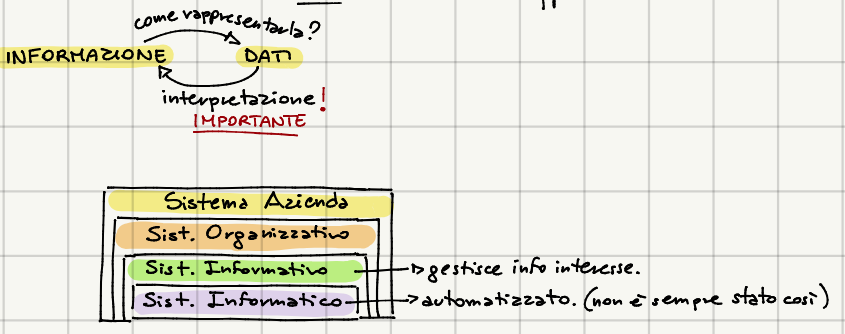
\includegraphics[width=0.7\linewidth]{schema1.png}
    \end{figure}
    \textbf{Gestire delle informazioni} vuol dire raccolta, acquisizione, archiviazione, conservazione, elaborazione, scambio, sincronizzazione, etc...
    \item \textbf{Che cos'è una base di dati?} È un insieme \textbf{organizzato} di dati utilizzati per il \textbf{supporto allo svolgimento} delle attività di un ente ed è gestito da un Sistema di Gestione di Basi di Dati o \textbf{DataBase Management System (DBMS)}. Una base di dati può essere vista in due modi: In senso generico: è un insieme organizzato di dati, utilizzato a supporto delle attività di un'organizzazione. \textit{(Esempio: per un'università, la base di dati riguarda le carriere degli studenti, i voti, le iscrizioni; per un ospedale, i pazienti, le diagnosi, le terapie.) }; In senso tecnologico: la base di dati è il sistema che permette di gestire quei dati, cioè il software e l'infrastruttura che ne consentono utilizzo, interrogazione e conservazione.
    \item \textbf{Cos'è un DBMS?} È un sistema informatico che gestisce collezioni di dati \textbf{di grandi dimensioni (numerosi e complessi), persistenti (memorizzati in maniera durevole), condivisi (accessibili da più utenti con diversi livelli di visibilità e autorizzazione)} garantendo \textbf{privatezza (accesso regolato ai dati), affidabilità (sicuri, integri e consistenti in qualsiasi condizione), efficienza (utilizzo di tempo e memoria ottimali), efficacia (deve farmi risparmiare tempo).} Si basa sul concetto di \textbf{transazione}, che deve essere corretta, ed atomica, ovvero che a fronte di un malfunzionamento ci assicura che i dati non vengano persi. Le transazioni, inoltre, sono \textbf{concorrenti}, cioè l'effetto deve essere coerente (equivalente) per ciascuna transazione che avvenga in contemporanea. Una transazione deve essere con \textit{effetti definitivi.} (per i posteri, guardare i criteri ACID)
    \item \textbf{Sistema organizzativo e informativo}: ogni organizzazione ha un \textbf{Sistema Organizzativo} che è l'insieme di \textbf{risorse} e regole per lo svolgimento coordinato delle attività (processi) al fine del perseguimento degli scopi. Le risorse di un'azienda sono persone, denaro, materiali, \underline{informazioni}. Ogni organizzazione ha un \textbf{Sistema Informativo}, eventualmente non esplicitato nella struttura. Quasi sempre, il sistema informativo è di supporto ad altri sottosistemi, e va quindi studuiato nel contesto in cui è inserito. Il sistema informativo è di solito suddiviso in sottosistemi (in modo gerarchico o decentrato), più o meno fortemente integrati. Il sistema informativo è parte del sistema organizzativo, ed esegue e gestisce i processi informativi (cioè che coinvolgono le informazioni). \textbf{Il concetto centrale che va ricordato è che il sistema informativo è la parte dell'organizzazione che gestisce le informazioni di interesse.} Quando però questa gestione delle informazioni avviene in modo automatizzato, cioè tramite un elaboratore, allora si parla di \textbf{sistema informatico.} Il concetto di sistema informativo è indipendente da qualsiasi automatizzazione; esistono organizzazioni la cui ragion d'essere è la gestione di informazioni e che operano da secoli. Il termine “\textit{automatizzato}” significa infatti che non è più l'uomo, manualmente, a raccogliere, scrivere e organizzare i dati, ma che tale compito è affidato a un sistema tecnologico, un calcolatore. Oggi, praticamente sempre, quando si parla di sistema informativo, si intende di fatto un sistema informatico: la gestione manuale è stata sostituita quasi del tutto da quella automatizzata. In passato però non era così. Un esempio importante è l'anagrafe. L'anagrafe ha sempre avuto il compito di gestire informazioni fondamentali come nascite, decessi, residenze, matrimoni, ecc. In origine non esistevano sistemi informatici, e tutto questo veniva registrato a mano in grandi registri cartacei. Chiunque abbia avuto modo di vederli, sa che si trattava di veri e propri mega-libri, compilati a penna, nei quali si scrivevano i dati con dovizia di particolari. Quella era già gestione dell'informazione, solo che avveniva senza sistemi informatici. Questo esempio mostra chiaramente che un sistema informativo può esistere anche senza strumenti tecnologici; semplicemente, oggi, tali strumenti sono diventati indispensabili e quindi i termini “sistema informativo” e “sistema informatico” tendono ad essere usati quasi come sinonimi.
    \textbf{Sistema informatico:} è la porzione automatizzata del sistema informativo. È la parte del sistema informativo che gestisce informazioni con tecnologia informatica. 
    \begin{figure}[h!]
        \centering
        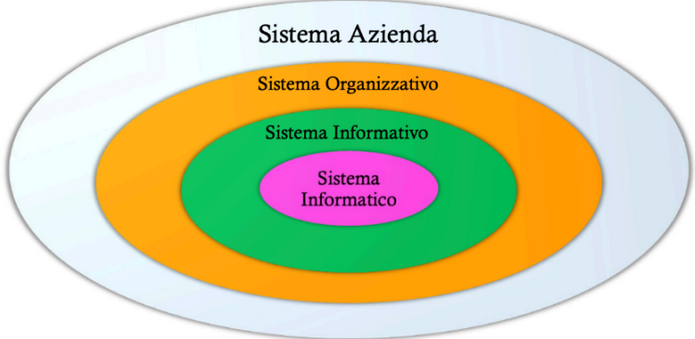
\includegraphics[width=0.5\linewidth]{ger1.png}
    \end{figure}
\end{itemize}
\subsection{Modellazione dei dati}
Una \textbf{base di dati} è un insieme organizzato di dati; per organizzare i dati serve un \textbf{modello di dati}. Un \textbf{modello dei dati} è un insieme di concetti utilizzati per organizzare i dati di interesse e descriverne la struttura in modo che essa risulti comprensibile ad un elaboratore.

\textbf{Modelli logici:} organizzano i dati in modo strutturato ma ancora astratto. Esempio: il modello relazionale, che rappresenta i dati con tabelle e relazioni.
\textbf{Modelli concettuali:} ancora più astratti, descrivono i concetti fondamentali di un dominio
indipendentemente dal modello logico. \textit{Esempio: modello entità-relazione (E-R), che rappresenta concetti come Studente, Corso e la relazione frequenta. }
Serve per dare una visione ad alto livello, più intuitiva, del dominio di interesse.

\subsubsection{Schema, Istanza e Architettura delle basi di dati}
\textbf{Schema: }\begin{itemize}
    \item Lo schema descrive la struttura della base di dati.
    \item È sostanzialmente invariante nel tempo: quando progetto uno schema cerco che sia definitivo. Non è “scolpito nella pietra” (può cambiare), ma la buona progettazione serve proprio a ridurre al minimo le modifiche. Perché? Perché se cambio lo schema, devo poi aggiornare tutte le istanze e adattare tutte le query collegate. \textit{Esempio: se aggiungo una colonna “secondo nome” alla tabella degli studenti, devo aggiornare ogni riga della tabella. Con basi di dati grandi, ciò diventa costoso.}
\item In sintesi: lo schema è la descrizione formale della struttura dei dati (es. attributi delle tabelle, tipi di dato, relazioni tra entità).
\end{itemize}
\textbf{Istanza:} L'istanza è l'insieme dei valori attuali contenuti nella base di
dati. Sono i dati veri e propri, che possono cambiare nel tempo. Esempio: aggiungere uno studente, modificare un voto, cancellare un record. Le istanze cambiano quotidianamente, mentre lo schema
dovrebbe rimanere stabile. 

\emph{Schema = struttura dei dati. Istanza = valori memorizzati.}

Il concetto di schema e istanza non vale solo per il modello logico (relazionale), ma anche per il livello concettuale. In un diagramma E-R (Entità-Relazioni) lo \textbf{schema} è costituito dalle \textbf{entità} (rettangoli) e dalle \textbf{relazioni} (rombi) che collegano le entità. L’\textbf{istanza} è costituita dalle \textbf{occorrenze} delle entità e dalle \textbf{coppie} (o tuple) che formano le \textbf{relazioni}.

\begin{figure}[h!]
    \centering
    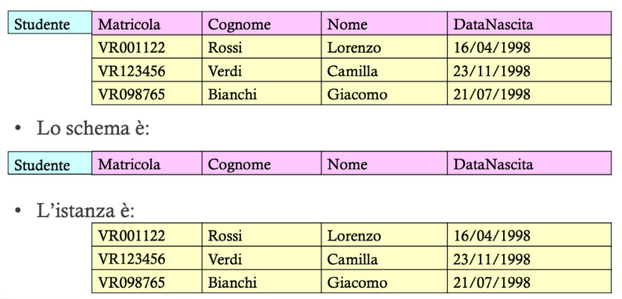
\includegraphics[width=0.5\linewidth]{immagine.png}
\end{figure}

Esempi:\begin{itemize}
    \item Entità Studente → ciascuno studente reale è un'istanza.
    \item Entità Docente → ciascun professore è un'istanza.
    \item Relazione Relatore di tesi → è rappresentata dalle coppie (Docente, Studente) che concretamente svolgono quella relazione.
\end{itemize}
\begin{figure}[h!]
    \centering
    
\includegraphics[width=0.25\linewidth]{er.png}
\end{figure}

\subsubsection{Architettura semplificata di un DBMS}
\begin{itemize}
    \item \textbf{Utente: interroga la base di dati o inserisce nuovi dati.}
 Esempio: uno studente si iscrive a un appello → inserimento di dati. Il docente controlla la lista degli iscritti → interrogazione della base di dati.

\item \textbf{Livello logico (schema logico):}
L’utente interagisce con le tabelle (modello relazionale). Scrive query SQL che operano sui dati organizzati in tabelle. Non si preoccupa di come i dati siano memorizzati fisicamente.

\item\textbf{Livello fisico (schema interno):} Descrive come i dati sono realmente memorizzati nei dispositivi (file, puntatori, strutture di archiviazione). Questo livello è gestito dal DBMS, non dall’utente.

\item \textbf{Indipendenza dei dati:} il livello logico è indipendente da quello fisico: una tabella è utilizzata nello stesso modo qualunque sia la sua realizzazione fisica. L’utente e il progettista interagiscono solo col modello logico (tabelle, attributi, tuple). Non devono preoccuparsi di come i dati siano fisicamente memorizzati. È il DBMS che si occupa di gestire la memorizzazione fisica. Per questo motivo, nello studio ci si concentra soprattutto sul modello relazionale e sulle query SQL: è il livello con cui realmente si interagisce.
\end{itemize}

\subsubsection{Utente, sistema informativo e modello relazionale}\begin{itemize}


\item\textbf{Interazione dell’utente con il DBMS:} L’utente che utilizza un DBMS (Database Management System) non interagisce con il modello concettuale in modo diretto. Può usarlo come documentazione per capire quali sono i concetti importanti. Quando interagisce, lo fa direttamente a livello logico, cioè lavora con le tabelle, le relazioni, i dati organizzati secondo lo schema logico. Il modello concettuale serve al progettista per rappresentare i concetti rilevanti del dominio, ma l’utente
finale non deve preoccuparsene.

\item\textbf{Sistema informativo e dati}: Un sistema informativo esprime l’informazione di interesse. Differenza tra dato e informazione: Dato → valore grezzo, singolo elemento. Informazione → interpretazione dei dati in un contesto applicativo, utile per prendere decisioni o
rispondere a domande concrete. Contesto applicativo: determina quali dati sono rilevanti. \textit{Esempio: memorizzare i dati degli studenti. Il numero di scarpe non è rilevante, a meno che non serva per un contesto particolare.}

\item\textbf{Modello di dati:} La base di dati è un insieme organizzato di dati, gestito da un DBMS. L’organizzazione dei dati è rappresentata tramite modelli di dati, che forniscono costrutti concettuali per strutturare le informazioni.Tipi di modelli di dati: \textbf{Concettuali} → rappresentano concetti importanti (E-R). \textbf{Logici} → rappresentano la struttura reale delle tabelle e delle relazioni (modello relazionale).
\item \textbf{Schema e istanza}
\textbf{Schema} → organizzazione dei dati secondo il modello scelto. \begin{itemize}[label=$\diamond$]
    \item Relazionale: struttura delle tabelle, attributi, tipi di dati.
    \item Concettuale: entità e relazioni.
\end{itemize}
\textbf{Istanza} → dati effettivi memorizzati. \begin{itemize}[label=$\diamond$]
\item Relazionale: tuple della tabella.
\item Concettuale: occorrenze delle entità e delle relazioni.
\end{itemize}
L’utente interagisce con lo schema logico, non con quello fisico, garantendo indipendenza dei dati.
\item \textbf{Modello relazionale di dati}: Proposto negli anni ’60 per favorire l’indipendenza dei dati: gli utenti non devono preoccuparsi di file o puntatori. Pubblicato negli anni ’70 e diventato operativo negli anni ’80 (1981) È il modello più utilizzato nella pratica (quasi il 99$\%$ dei DB reali). Si basa su due concetti principali: \begin{enumerate}
    \item Relazione matematica → insieme di tuple su uno o più domini.
    \item Tabella → rappresentazione concreta delle relazioni, con righe e colonne.
\end{enumerate}
\end{itemize}

\subsubsection{Concetto di relazione}
La parola relazione ha tre accezioni: \begin{enumerate}
    \item Matematica → sottoinsieme del prodotto cartesiano di domini.
    \item E-R (Entità-Relazione) → associazione tra entità (es. relatore di tesi e studente).
    \item Modello relazionale dei dati → tabella organizzata secondo domini e tuple.
\end{enumerate}
È importante capire il contesto per sapere a quale significato ci si riferisce.
\begin{itemize}
     
\item \textbf{Relazione matematica: } una relazione matematica è \emph{per definizione} il \textbf{prodotto cartesiano dei domini degli insieme in relazione.} \textit{Ad esempio:} 

Dominio $D_1 = \{1,2\}, D_2 = \{x,y,z\}$

Prodotto Cartesiano: $D_1 \times D_2 = \{ (1,x), (1,y), (1,z), (2,x),(2,y),(2,z)\}$ 

Una relazione $R \subseteq D1 \times D2 \to R = \{(1,x), (2,x), (2,z)\}$

\textbf{L'ordine dei valori nel prodotto cartesiano è posizionale.} 
\item \textbf{Relazione nel modello relazionale (Codd):} Codd introduce una variante della relazione matematica per rendere la relazione non posizionale: Nelle tabelle, \textbf{i valori non dipendono dalla posizione della colonna.} Ogni colonna ha un ruolo distinguibile tramite il nome, non tramite l’ordine. Questo semplifica le interrogazioni e la gestione dei dati: non occorre ricordare quale colonna rappresenta quale informazione. \textbf{Esempio tabella “partite”:} \begin{itemize}
    \item Colonne: squadra in casa, squadra ospite, goal squadra in casa, goal squadra ospite
\item Ogni dominio ha un ruolo distinto, identificabile dalla colonna, non dalla posizione.
\end{itemize}


\end{itemize}


%%%%%%%%%%%%%%%%%%%%%%%%%
\textbf{Relazione nel modello relazionale:} relazione matematica con una variante che mira a rendere la notazione NON posizionale. 

\textbf{\textit{Esempio: }} Partite $\subseteq$ string $\times$ string $\times$ int $\times$ int $\leftarrow$ A ciascun dominio viene associato un nome (\textbf{attributo}) che è unico nella relazione e descrive il "ruolo" (il significato) del dominio.

\begin{table}[h!]
    \centering
    \begin{tabular}{|c|c|c|c|}
    \hline
    \textbf{Squadra casa}     &  \textbf{Squadra fuori} & \textbf{Reti casa }&  \textbf{Reti fuori}\\
    \hline
    Milan & Inter & 2 & 0 \\
    \hline
    Roma & Lazio & 0 & 0 \\
    \hline
    Inter & Roma & 2 & 0 \\
    \hline
    Lazion & Milan & 0 & 0 \\
    \hline
    
    \end{tabular}
    \caption{Esempio non posizionale di relazione}
    \label{tab:esempiononrelaz}
\end{table}
Il significato della colonna è descritto dal nome della colonna stessa, quindi l'ordine della riga non è più rilevante nell'informazione $\to$ \textbf{Relazione NON posizionale.}

\textbf{Tabelle e relazioni (nel modello relazionale dei dati):}
<Domanda di Esame> quando una tabella rappresenta una relazione nel modello relazionale dei dati? \textit{(per i posteri, 1 Forma Normale)}
\begin{itemize}
    \item Una tabella rappresenta una relazione \textit{se} i valori di ogni colonna sono fra loro \textbf{omogenei}, perché appartengono allo stesso dominio.
    \item le righe della tabella sono tutte diverse tra loro, perché la relazione è un insieme, quindi ogni elemento(riga) è diverso tra loro.
    \item Le intestazioni di ogni colonna sono diverse perché se dò nomi uguali si torna ad una notazione posizionale, mentre io ne voglio una NON posizionale. 
\end{itemize}

Se una tabella rappresenta una relazione, abbiamo che l'ordinamento tra le righe è \textbf{irrilevante}, perché \textit{essendo un insieme, non importa l'ordine}. Anche l'ordinamentro tra le colonne è \textbf{irrilevante}, siccome vogliamo una notazione non posizionale, quindi quando ogni colonna ha il suo nome posso mescolarle e non cambia nulla.  \textbf{RICORDA: }\textit{la relazione è un insieme.}

Nel modello relazionale ogni riga si chiama \textbf{\textit{tupla}}, ed ogni valore nella tupla lo recupero indicando il valore dell'attributo. Ad esempio, nella tabella \ref{tab:esempiononrelaz}, se t è la prima tupla, allora \textit{t[squadraCasa]} = "Milan".

In una relazione un \textbf{collegamento è basato sui valori}, infatti, ad esempio, posso collegare la prima squadra della tabella \ref{tab:esempiononrelaz} con la tabella
\begin{table}[h!]
    \centering
    \begin{tabular}{|c|c|c|}
    \hline
    \textbf{NomeSquadra} & \textbf{Anno} &\textbf{Città} \\
    \hline
        Milan & 1899 & Milano \\
        \hline
        ... & ... & ...\\
        \hline
    \end{tabular}
    \caption{Squadre}
    \label{tab:squadre}
\end{table}

\newpage
\subsection{DEFINIZIONI relative al MODELLO RELAZIONALE DEI DATI}
\begin{itemize}
    \item \textbf{Grado:} numero di colonne di una relazione;
    \item \textbf{Cardinalità:} numero di tuple dell'istanza di una relazione.

    \item \textbf{Schema di relazione:} \small(\textit{Schema:} struttura, organizzazione dei dati.) \normalsize Descrive la STRUTTURA  e si indica $R(X)$ dove $R$ è il nome della relazione, $X$ è l'insieme degli attributi, quindi $X = {A_1, A_2, ..., A_n}$; Ad ogni attributo è associato un dominio. 
    
    \textit{\textbf{Esempio:}} $Studente(Matricola,Cognome, Nome, DataNascita)$
    \item \textbf{Schema di base di dati:} un'insieme di schemi di relazione con nomi diversi.
    \begin{equation*}
        \boldsymbol{R}= \{  R_1(X_1), R_2(X_2), ..., R_n(X_n) \}
    \end{equation*}

    \textit{Esempio:} 
    \begin{align*}
        \boldsymbol{R} = \{ Studente(Matricola, Cognome, Nome, Datanascita),\\
        Docente(Codice, Cognome, Nome, NumTel), \\ Supervisore(MatrSt CodDoc, DataInizio)\}
    \end{align*}
    \item \textbf{Tupla:} una tupla su in insieme di attributi $X$ è una \textit{funzione} che associa a ciascuno degli attributi $A$ in $X$ un valore del dominio di A. \textit{Esempio:} $t[A]$ denota il valore della tupla $t$ sull'attributo a
    \item \textbf{(ISTANZA di) RELAZIONE:} \small Quando parliamo di relazione spesso parliamo di istanza di relazione. \normalsize È data dal contenuto della relazione, cioè è formata dall'\textit{insieme delle tuple della relazione.}
    \item \textbf{Istanza di una relazione su uno schema $R(X)$}: insieme $r$ di tuple su X.
    Esempio: dato lo schema di relazione Studente(Matricola, Cognome, Nome, DataNascita), l'istanza potrebbe essere \begin{align*}
        r = \{(VR000001, Rossi, Mario, 12/04/2005), \\(VR000002, Gialli, Lucia, 27/0/2004),\\ (VR000003, Verdi, Luca, 21/08/2006)\}
    \end{align*}
    \item \textbf{(ISTANZA di) BASE di DATI:} istanza di basi di dati su uno schema \begin{equation*}
        \boldsymbol{R}= \{  R_1(X_1), R_2(X_2), ..., R_n(X_n) \}
    \end{equation*} è data dall'insieme di (istanze di) relazioni $r = 
\{ r_1, r_2, ..., r_n\ \}$
 \begin{align*}
        \boldsymbol{R} = \{ Studente(Matricola, Cognome, Nome, Datanascita), \\ Docente(Codice, Cognome, Nome, NumTel), \\ Supervisore(MatrSt CodDoc, DataInizio)\}
    \end{align*}
    quindi
    
    \begin{align*}
        r = \{ \quad \{(VR000001, Rossi, Mario, 12/12/2005), \quad (VR00002, Gialli, Lucia, 16/01/2005)\},\quad \\ \{(DO1, Oliboni, Barbara, 045 ...), \quad (DO2, Quintarelli, Elisa, 045 ...)\},\quad \\ \{VR00001, DO1, 01/10/2025), \quad (VR005, DO2, 20/09/2025)\} \quad \}
    \end{align*}
    
    Avremmo quindi le seguenti tabelle:
    
\noindent
\begin{minipage}{.4\textwidth}
  \centering
    \begin{tabular}{|c|c|c|c|}
        \hline
        \textbf{Matricola} & \textbf{Cognome} & \textbf{Nome} & \textbf{DataNascita}\\
        \hline
         VR00001 & Rossi & Mario & 12/12/2005 \\
         \hline
         VR00002 & Gialli & Lucia & 16/01/2005 \\
         \hline
        \end{tabular}
  \captionof{table}{Studente}
\end{minipage}%
\hfill
\begin{minipage}{.4\textwidth}
  \centering
       \begin{tabular}{|c|c|c|c|}
        \hline
          \textbf{Codice} & \textbf{Cognome} & \textbf{Nome} & \textbf{NumTel} \\
          \hline
          DO1 & Oliboni & Barbara & 045 ... \\
          \hline
          DO2 & Quintarelli & Elisa & 045... \\
          \hline
        \end{tabular}
\captionof{table}{Docente}
\hspace{1em}
\end{minipage}

\noindent
\begin{minipage}{.4\textwidth}
  \centering
    \begin{tabular}{|c|c|c|}
        \hline
         \textbf{MatrSt} & \textbf{CodDoc} & \textbf{DataInizio} \\
         \hline
         VR00001 & DO1 & 01/10/2025 \\
         \hline
         VR00002 & DO2 & 20/09/2025\\
         \hline
        \end{tabular}
  \captionof{table}{Supervisore}
\end{minipage}%
\hfill
\begin{minipage}{.4\textwidth}
  \centering
       \begin{tabular}{|c|}
        \hline
          \textbf{Rappresentante} \\
          \hline
            VR000002 \\
          \hline
        \end{tabular}
\captionof{table}{Rappresentante}
\end{minipage}

    Le informazioni delle tabelle sono collegate, e le relazioni possono essere anche con un solo attributo e si basano sui valori.

    \textbf{Lo schema della Base di Dati impone una struttura rigida definita a priore.} Tutti i dati inseriti nella base di dati infatti devono rispettare quello schema, una volta deciso. Questo significa che le tuple che posso inserire nella mia base di dati devono rispettare la struttura che ho definito. 
    \end{itemize}

    Per alcune tuple, potrei non avere il valore di qualche attributo. $\to$ \textbf{Informazione incompleta}
    
    Ad esempio:
    \begin{table}[h!]
        \centering
        \begin{tabular}{|c|c|c|c|c|}
        \hline
        \textbf{Matricola} & \textbf{Cognome} & \textbf{PrimoNome} & \textbf{SecondoNome} & \textbf{DataNascita}\\
        \hline
         VR00001 & Rossi & Mario & Francesco & 12/12/2005 \\
         \hline
         VR00002 & Gialli & Lucia & $\boldsymbol{NULL}$ & 16/01/2005 \\
         \hline
        \end{tabular}
        \caption{Studente}
        \label{tab:valorinull}
    \end{table}

\textit{Se non so un valore non metto testo "Placeholder" perché una tupla potrebbe aver bisogno di usare proprio quel valore, quindi non è consigliato cercare una stringa.} La soluzione è scegliere un \textbf{VALORE NULLO:} denota l'assenza di un valore nel dominio, NON È UN VALORE DEL DOMINIO. Quindi in una colonna o abbiamo un valore del dominio, o valore nullo.

\textbf{Tipi di valori nulli:}
\begin{itemize}
    \item \textbf{Valore sconosciuto:} il valore esiste, ma a noi non è noto.
    \item \textbf{Valore inesistente:} il valore non esiste nella realtà modellata.
    \item \textbf{Valore senza informazione:} il valore può esistere o non esistere e se esiste non sappiamo quale sia. (Caso più generale). \textit{Nei DBMS un valore NULL è interpretato come questo caso, ovvero l' \textbf{"OR"} logico dei due precedenti casi}.
\end{itemize}

\textbf{Esempio:}
    
\noindent
\begin{minipage}{.4\textwidth}
  \centering
    \begin{tabular}{|c|c|c|c|}
        \hline
        \textbf{Codice}&\textbf{Nominativo}&\textbf{Telefono}&\textbf{DataNascita} \\ 
        \hline
        NULL & A.A & 045 ... & 12/06/2000 \\
        \hline
        PO2 & B.B & NULL & 15/05/2005 \\
        \hline
        PO3 & C.C & 045... & NULL \\
        \hline
        \end{tabular}
  \captionof{table}{Paziente}
\end{minipage}%
\hfill
\begin{minipage}{.4\textwidth}
  \centering
   \begin{tabular}{|c|c|c|}
    \hline
    \textbf{Codice} & \textbf{Nominativo}& \textbf{Specializzazione} \\
    
    \hline  
         MO1 & NULL & NULL \\
         \hline  
         MO2 & E.E & Ortopedia \\
         \hline  
         MO3 & F.F & Chirurgia \\
         \hline  
         NULL & E.E & NULL \\
         \hline
        \end{tabular}
\captionof{table}{Medico}
\hspace{1em}
\end{minipage}
\begin{table}[h!]
    \centering
    \begin{tabular}{|c|c|c|}
    \hline
        \textbf{CodP}& \textbf{CodM} & \textbf{Motivo}\\
        \hline
        PO2 & MO2 & NULL \\
        \hline
        NULL & MO1 & Artrite \\
        \hline
        PO3 & NULL & NULL \\
        \hline
    \end{tabular}
    \caption{In cura}
\end{table}

\textit{Osservazioni relazione "paziente"}

\mybox{Se non ha un codice la prima tupla in paziente, non potrò mai connetterlo con la base di dati, quindi è un problema; non posso lasciare NULL il codice. Il numero di telefono, invece, non crea problemi; tantomeno la data di nascita; non creano problemi nello schema attuale della base di dati e delle sue istanze se assume valore NULL.}

\textit{Osservazioni relazione "medico"}

\mybox{Nel caso della prima tupla, la coppia null nominativo-specializzazione è un problema, perché \textbf{ci sono così tanti valori nulli che la tupla non esprime alcuna informazione!}
NEL CASO  DELLA SECONDA E QUARTA TUPLA IL NULL CREA PROBLEMI PERCHÉ POTREBBE ESSERE LA STESSA TUPLA.}

\textbf{Si possono/devono imporre restrizioni sulla presenza di valori nulli.} Nella definizione dello schema della relazione è possibile/auspicabile specificare su quali attributi non sono (o sono) ammessi valori nulli. 
Ad esempio, se decido che posso NON avere il numero telefono, potrebbe essere \begin{equation*}
    PAZIENTE(Codice,Nominativo,Telefono^*,DataNascita)
\end{equation*}
Se su un attributo metto un asterisco, significa che sono ammessi valori nulli, altrimenti NON sono ammessi. Secondo quest'ultimo schema, nella tabella paziente l'unica tupla ammessa è la seconda. 

\section{Modello relazionale}
\subsection{Vincoli di integrità:}
\textbf{Vincoli di integrità:} descrivono le proprietà che devono essere soddisfatti dai dati (cioé le sue istanze) all'interno della nostra base di dati per rappresentare \textbf{informazioni corrette}. Ad esempio scrivere \begin{align*}
    STUDENTE(Matricola, Cognome, Nome, DataN, NumTel, Indirizzo*)
\end{align*} significa affermare che nell'istanza di uno studente \textit{solo l'indirizzo} può essere non inserito, cioè NULL, mentre tutti gli altri devono avere un valore per essere corretti. 
Un \textbf{VINCOLO} è una funzione booleana che associa ad ogni istanza il valore \textit{vero o falso.} Quando paarlo di integrità, parlo di \textbf{qualità dei dati}, cioè di rappresentare in maniera \textbf{corretta e completa} i dati memorizzati. Un altro valore di integrità indica quale può essere il valore assunto da un determinato attributo. \textit{Ad esempio, un voto di un esame può andare da 18 a 30.} Quindi il vincolo di integrità può \textbf{specificare anche il dominio.}

\textbf{Tipi di vincoli di integrità}

\textit{Posso classificarli sulla base degli elementi coinvolti, e abbiamo due categorie:}
\begin{itemize}
    \item \textbf{Vincoli INTRA-relazionali:} cioè sono vincoli riferiti ad una singola tabella alla volta, cioè su \textit{singole relazioni}. Tra questi abbiamo: \begin{enumerate}
        \item \textbf{Vincolo di TUPLA:} la valutazione avviene su ciascuna tupla indipendentemente dalle altre. Specifico una proprietà che vado a verificare su ogni singola tupla. La validazione della tupla e l'accettazione di questa quindi dipende singolarmente dai valori contenuti in essa. 

        \textit{Ad esempio:} $voto\geq 18 \land voto \leq 30 \land EsameSuperato = SI$.

        \item \textbf{Vincolo su VALORI (di DOMINIO):} vincolo riferito ad un singolo valore. 

        \textit{Esempio:} $Settimana \geq 1 \land Settimana \leq 40 $.

        \item \textbf{Vincolo di CHIAVE:} permette di specificare qual è l'insieme di attributi che identificano in maniera univoca ogni singola tupla. La chiave primaria è l'insieme \emph{minimo} di attributi, che non possono assumere valore NULL. \textbf{La chiave identifica UNIVOCAMENTE ogni tupla.}

        \textbf{Esempio:} $STUDENTE(\underline{matricola}, cognome, nome, ...)$
    \end{enumerate}

    
\textit{Esempio: } $CORSO(\underline{codice}, titolo, descrizione*, CFU)$ dove $CFU \geq 2 \land CFU \leq 12.$
    \begin{table}[h!]
    \centering
    \begin{tabular}{|c|c|c|c|}
    \hline
        \textbf{\underline{Codice}} &  \textbf{Titolo} & \textbf{Descrizione} & \textbf{CFU} \\
        \hline
        BD1 & Basi di Dati &  ... & 6 \\
        \hline
        ALGO & Algoritmi & \textit{Descrizione} &  12 \\
        \hline
        
    \end{tabular}
    \caption{Tabella Corso: esempio vincoli intrarelazionali}
    \end{table}
    
    \item \textbf{Vincoli INTER-relazionali:} fanno riferimento a più relazioni. \textbf{Vincoli di integrità referenziale.}

    \textit{Esempio sulla tabella indicata sopra, non esiste l'esame $BD2$, quindi non posso referenziarlo.}
    \begin{table}[h!]
    \centering
    \begin{tabular}{|c|c|c|c|}
    \hline
        \textbf{\underline{Matricola} }&  \textbf{Codice Corso (FK)} & \textbf{Voto} & \textbf{Data} \\
        \hline
        VR01 & BD1 &  30 & 02/09/2025 \\
        \hline
        VR02 & \cancel{BD2} &  26 & 03/09/2025 \\
        \hline
        
    \end{tabular}
    \caption{Tabella Esame: esempio vincoli interrelazionali}
\end{table}
\end{itemize}

\mybox{
\textbf{\underline{Possibile domanda d'esame}}

\textit{Si dica che cosa sono i vincoli di integrità specificando brevemente le due categorie.}}

\subsection{Chiavi}
\textbf{Vincolo di chiave:} intuitivamente una \textbf{CHIAVE} è uno o un insieme di attributi utilizzato per 
\textbf{identificare univocamente le tuple di una relazione.}
\newpage
\textit{Esempio con paziente dell'ospedale:}
\begin{table}[h!]
    \centering
    \begin{tabular}{|c|c|c|c|c|}
         \hline
         \textbf{\underline{Codice}} & \textbf{Cognome} & \textbf{Nome} & \textbf{CittaNascita} & \textbf{DataNascita} \\
         \hline
         PAZ011 & Verdi & Giulia &  Verona & 02/03/1990 \\
         \hline
         PAZ012 & Neri & Giulia &  Milano & 18/12/1989 \\
         \hline
         PAZ013 & Verdi & Greta &  Verona & 02/03/1990 \\
         \hline
    \end{tabular}
    \caption{Tabella Paziente: esempio di vincoli di chiave.}
\end{table}

Il \textbf{CODICE} identifica univocamente i pazienti in questo esempio. Anche i dati anagrafici \{ Cognome, Nome, DataNascita \} identificano i pazienti.

\mybox{\textbf{DEFINIZIONE di CHIAVE:} la chiave di una relazione è un \textit{insieme di attributi} che serve ad identificare \textbf{UNIVOCAMENTE} le tuple della relazione e che garantisce le seguenti proprietà: \begin{enumerate}
    \item \textbf{UNICITÀ:} in una qualunque istanza della relazione non possono esistere due tuple distinte, la cui restrizione alla chiave sia uguale, cioè che abbiano gli stessi valori sugli attributi della chiave.
    \begin{align}
        t_1[k] = t_2[k] \Rightarrow t_1[x] = t_2[x]
    \end{align}
    \item \textbf{MINIMALITÀ:} non deve essere possibile sottrarre alla chiave un attributo senza che la condizione di unicità cessi di valere. Cioè, \textit{una chiave non contiene un'altra chiave.}
\end{enumerate}}

\textbf{CHIAVE E SUPERCHIAVE:}\begin{itemize}
    \item Un insieme $K$ di attributi è \textbf{SUPERCHIAVE} per $r$ se $r$ NON contiene due tuple distinte $t_1$ e $t_2$ con $t_1[k] = t_2[k]$.
    \item Un insieme $K$ di attributi è \textbf{CHIAVE} per $r$ se è una \textbf{SUPERCHIAVE MINIMALE} per $r$ (cioè non contiene un'altra superchiave).
\end{itemize}

\textit{Esempio con paziente dell'ospedale:}
\begin{table}[h!]
    \centering
    \begin{tabular}{|c|c|c|c|c|}
         \hline
         \textbf{Codice} & \textbf{Cognome} & \textbf{Nome} & \textbf{CittaNascita} & \textbf{DataNascita} \\
         \hline
         PAZ011 & Verdi & Giulia &  Verona & 02/03/1990 \\
         \hline
         PAZ012 & Neri & Giulia &  Milano & 18/12/1989 \\
         \hline
         PAZ013 & Verdi & Greta &  Verona & 02/03/1990 \\
         \hline
    \end{tabular}
    \caption{Tabella Paziente: esempio di chiave e superchiave.}
\end{table}

\begin{itemize}
    \item In questa tabella \emph{\{Codice\}} è una chiave e  una superchiave, e contiene un solo attributo, cioè è un attributo minimale, quindi è chiave. 
    \item Mentre \emph{\{Codice, DataNascita\}} non è una chiave perché è superchiave, ma non è minimale. 
    \item È una superchiave anche \emph{\{Cognome, Nome, DataNascita\}} , ma non è minimale, perché posso togliere, ad esempio, la data di nascita, ed ho ancora valori univoci; non è minimale e quindi \textit{non è chiave.} 
    \item \emph{\{Cognome, Nome\}} è superchiave e minimale, quindi è chiave.
\end{itemize}

\mybox{\textbf{VERO O FALSO riassuntivo:}\begin{itemize}
    \item \textbf{Ogni relazione ha almeno una chiave}, \textbf{VERO}, poiché una relazione è un insieme, quindi male che vada ho tutti gli attributi come chiave. 
    \item Ogni relazione ha \textit{esattamente} una chiave? \textbf{FALSO}.  
    \item Ogni attributo della appartiene al massimo ad una chiave. FALSO. Una chiave può essere sottoinsieme di un'altra. \textbf{FALSO}. 
    \item Può esistere una chiave che coinvolge tutti gli attributi. \textbf{VERO.}
\end{itemize}}

\textbf{\underline{CHIAVE PRIMARIA}:} chiave su cui \textit{non sono ammessi valori nulli.}

Si indica sottolineando l'insieme di attributi. \begin{align*}
    STUDENTE (\underline{Matricola}, Cognome, Nome, DataNascita)\\
    PRODOTTO (\underline{Nome, Linea}, Descrizione, Prezzo) \\
    ESAME (\underline{MatricolaStudente, CodiceCorso}, Voto, Data)
\end{align*}

Quando come chiave primaria ho una coppia di attributi, è la coppia di valori che non si può ripetere, mentre i singoli sì. Cioé, nell'esempio sopra, nel caso dell'esame si può ripetere la matricola poiché si verbalizzano più esami, ma lo stesso esame è verbalizzato solo una volta per lo stesso studente. Cioè, data la la chiave primaria $(\underline{MatricolaStudente, CodiceCorso})$, le istanze $\{(ST01,BD1),(ST01,ALGO),(ST02,BD1)\}$ sono valide, mentre non lo sarebbe ripetere $\{(ST01,BD1),(ST01,BD1)\}$.

\subsection{Vincoli di integrità referenziale}
Lo scopo è quello di rappresentare informazioni \textbf{coerenti.} Vengono usati in particolare i valori delle chiavi primarie.

\textit{Esempio:}
\begin{align*}
    PAZIENTE(\underline{Codice}, Cognome, Nome, DataNascita, CodMedico) \\ MEDICO(\underline{Codice}, COgnome Nome, Ospedale, Reparto) \\
    REPARTO (\underline{Ospedale, Reparto}, Indirizzo, Telefono, COD\_Primario)
\end{align*}

\begin{table}[h!]
    \centering
    \begin{tabular}{|c|c|c|c|c|}
    \hline
        \textbf{Codice}& \textbf{Cognome }& \textbf{Nome} & \textbf{DataNascita} & \textbf{ CodiceMedico} \\
        \hline
        PAZ01 & Verdi & Giulia & 12/12/2004 & MED03 \\
        \hline
        PAZ02 & Neri & Giulia & 10/12/2005 & MED02 \\
        \hline
        PAZ03 & Verdi & Greta & 12/12/2004 & MED03 \\
        \hline
    \end{tabular}
    \caption{Paziente}
\end{table}


\begin{table}[h!]
    \centering
    \begin{tabular}{|c|c|c|c|c|}
    \hline
        \textbf{Codice}&\textbf{ Cognome} &\textbf{ Nome} &\textbf{ Ospedale} & \textbf{Reparto} \\
        \hline
        MED01 & Rossi & Mario & BR & Ostetricia \\
        \hline
        MED02 & Bronchi & Lucia & BT & Ostetricia \\
        \hline
        MED03 & Neri & Sara &  BT & Ostetricia \\
        \hline
        MED04 & Gialli & Andrea & Negrar & Ostetricia \\
        \hline
    \end{tabular}
    \caption{Medico}
\end{table}

\begin{table}[h!]
    \centering
    \begin{tabular}{|c|c|c|c|c|}
    \hline
        \textbf{Ospedale} & \textbf{Reparto} & \textbf{Indirizzo} & \textbf{Telefono} & \textbf{COD\_Primario} \\
        \hline
        BR & Ostetricia & ... & ... & MED01 \\
        \hline
        BT & Ostetricia & ... & ... & MED03 \\
        \hline
        Negrar & Ostetricia & ... & ... & MED04 \\
        \hline
    \end{tabular}
    \caption{Reparto}
\end{table}

I vincoli di integrità referenziale in questo esempio sono:

\textbf{TABELLE INTERNE $\to$ TABELLE ESTERNE}
\begin{itemize}
    \item $PAZIENTE.CodMedico \to MEDICO.Codice$
    \item $MEDICO.[Ospedale, Reparto] \to REPARTO.[Ospedale, Reparto]$
    \item $REPARTO.COD\_Primario \to MEDICO.Codice$
\end{itemize}


\mybox{\textbf{VINCOLO DI INTEGRITÀ REFERENZIALE (O DI FOREIGN KEY):}

Un vincolo di integrità referenziale fra gli attributi $X$, di una relazione $R_1$ e un'altra relazione $R_2$ impone ai valori su $X$ in $R_1$ di comparire come valori della chiave primaria di $R_2$. \begin{itemize}
    \item $R_1 \to$ \textbf{TABELLA INTERNA}, in cui specifico il vincolo di integrità referenziale.
    \item $R_2 \to$ \textbf{TABELLA ESTERNA}
\end{itemize}

\textbf{\textit{N.B.1 nei vincoli su più attributi conta l'ordine.}}

\textit{\textbf{N.B.2} Il valore dell'attributo Foreign Key può anche assumere valore NULL (se concesso dallo schema) qualora non vi sia ancora un collegamento con un altro valore. Deve rispettare i vincoli di integrità, infatti, solo se non è NULL.}
}

A livello di SQL, si possono scegliere politiche di reazione alla violazione dei vincoli di integrità referenziale. Ad esempio, qualora una tupla esterna viene referenziata, bisogna aggiornare le tuple interne che prima la referenziavano. Le modifiche che violano l'integrità referenziali possono essere sia della tabella interna, che di quella esterna.

 \par\rule{\textwidth}{0.5pt} 
 
\textit{ \textbf{Esercizio 1:} definire un modello relazionale dei dati per organizzare i dati di una clinica privata in cui lavorano degli infermieri. Ogni infermiere è associato ad un reparto ed ha un codice fiscale, nome, cognome data di nascita. Per i reparti si memorizzino il codice (identificativo)  il nome, il piano, il caporeparto (che è un infermiere) e il primario che è un medico. Di un medico si conoscono il codice (identificato), cognome, nome e specializzazione.}

\begin{align*}
    \textbf{INFERMIERE}(\quad\quad \underline{CF\_Infermiere}, Nome, Cognome, DataNascita,\quad \\ CodiceReparto(FK)\to REPARTO.CodiceReparto  \quad)\\
    \textbf{REPARTO}( \quad \underline{CodiceReparto}, Nome, Piano, Caporeparto (FK \to Infermiere.CF\_Infermiere),\quad \\CodicePrimario(FK \to Medico.CodiceMedico) \quad  ) \\
    \textbf{MEDICO}(\underline{CodiceMedico}, Cognome, Nome, Specializzazione)
\end{align*}

 \par\rule{\textwidth}{0.5pt} 

\textit{\textbf{Esercizio 2:} Ogni infermiere è associato ad un reparto ed ha CF, nome cognome e data di nascita.}
 
\textit{Per i reparti si memorizzano il codice, il nome, il piano e il minimo di posti letto.}
 
\textit{Per ogni letto si memorizza il reparto in cui si trova, il numero della stanza, il numero di letto e il suo tipo.
} 
\textit{Per ogni medico si memorizzano il reparto in cui lavora e le info personali tra cui codice, nome, cognome , la specializzazione, indirizzo e il numero di telefono (fisso e mobile).
} 
\textit{Il lavoro del reparto è organizzato in turni che hanno una data e un orario di inizio.}

\textit{Ogni reparto ha un medico come primario ed un infermiere come caporeparto (il caporeparto cambia ad ogni turno).}

\begin{align*}
    INFERMIERE(\underline{CF},Nome, Cognome, DataNascita, CodReparto \to REPARTO.CodReparto) \\
    REPARTO(\underline{CodReparto}, Nome, Piano, NumeroLetti, CodPrimario \to MEDICO.CodMedico) \\
    MEDICO (\underline{CodMedico}, Nome, Cognome, Specializzazione, Indirizzo, TelFisso, TelMob, \quad \\ CodReparto \to REPARTO.CodReparto)
    \\ LETTO ( \underline{CodReparto \to REPARTO.CodReparto, NumStanza, NumLetto}, Tipo)
    \\ TURNO (\underline{Data, Ora, CodReparto \to REPARTO.CodReparto, }, CodInfermiere \to INFERMIERE.CF)
\end{align*}
\par\rule{\textwidth}{0.5pt} 

\newpage
\begin{figure}[h!]
    \centering
    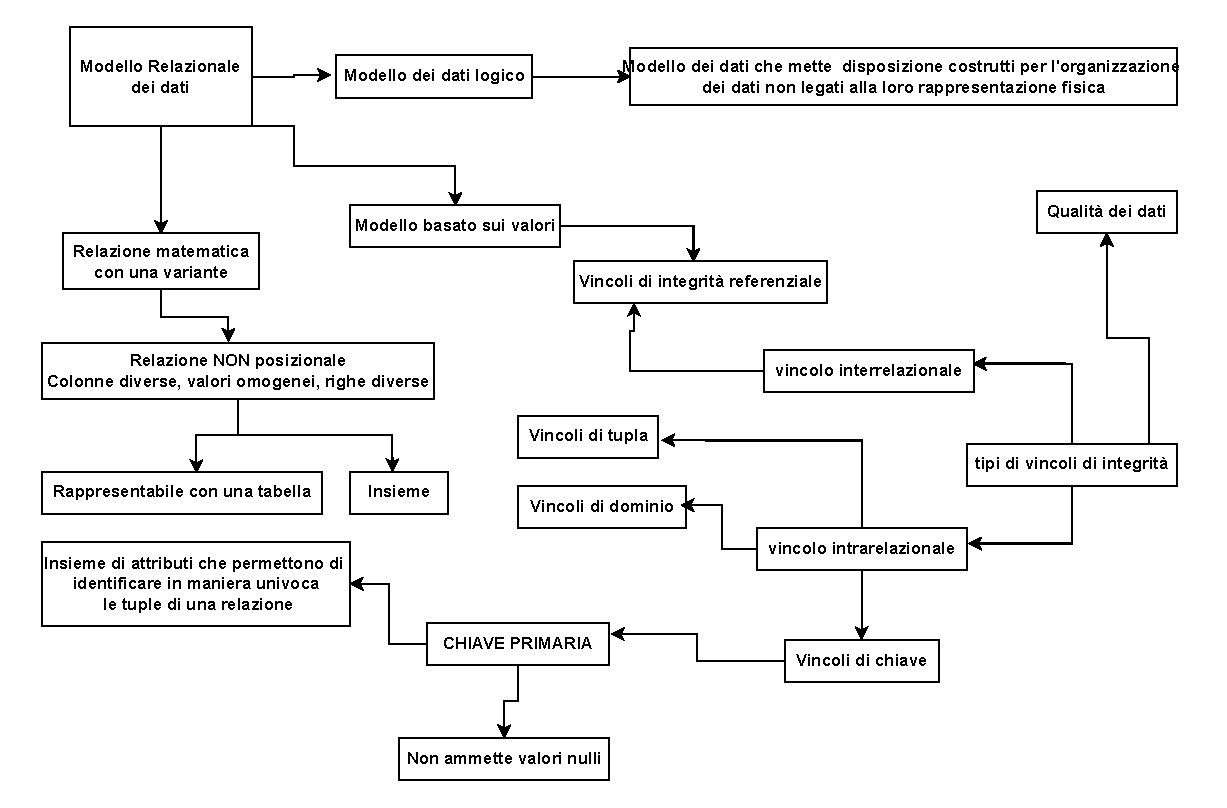
\includegraphics[width=1\linewidth]{SchemaBD1.pdf}
    \caption{Schema riassuntivo del modello relazionale}
\end{figure}

\newpage
\section{Algebra relazionale}
\textbf{Classificazione dei linguaggi:} \begin{itemize}
    \item \textbf{Linguaggi FORMALI:} Come l'algebra relazionale.
    \item \textbf{Linguaggi COMMERCIALI:} Come l'SQL (Structured Query Language).
\end{itemize}
Inoltre i linguaggi possono essere: \begin{itemize}
    \item \textbf{DICHIARATIVI: }specificano le proprietà del risultato, cioè "che cosa" voglio ottenere. SQL è un linguaggio dichiarativo.
    \item \textbf{PROCEDURALI: }specificano le modalità di generazione del risultato, cioè "come" ottenerlo, quali sono i passaggi. L'algebra relazionale è un linguaggio procedurale.
\end{itemize}

L'Algebra Relazionale quindi è un linguaggio \textit{formale e procedurale}, composto da un insieme di \textbf{operatori}, che producono \textbf{relazioni} e che possono essere composti.
\subsection{Operatori dell'algebra relazionale}
\begin{itemize}
    \item \textbf{OPERATORI INSIEMISTICI:}

    Le relazioni sono insiemi, si possono applicare solo a relazioni definite sugli stessi attributi. $R_1$ e $R_2$ devono essere \textbf{COMPATIBILI} quindi devono avere lo \textbf{stesso grado} e \textbf{domini ordinatamente dello stesso tipo.}
    
    \begin{itemize}
        \item \textbf{UNIONE} $R_1 \cup R_2$. Mette insieme tutte le tuple. 
        
        L'unione di due relazioni $r_1$ ed $r_2$ (istanze) definite sullo stesso insieme di attributi $X$, $r_1 \cup r_2$ è una relazione ancora su $X$ contenente tutte le tuple che appartengono ad $r_1$, oppure ad $r_2$, oppure ad entrambe.

        \textit{Esempio:}

 \begin{minipage}{.2\textwidth}
  \centering
            \begin{tabular}{|c|c|c|}
                 \hline
                 \textbf{Matricola} & \textbf{Nome} & \textbf{Età} \\
                 \hline
                 7274 & Rossi & 42 \\
                 \hline
                 7432 & Neri & 54\\
                 \hline
                 9824 & Verdi & 45 \\
                 \hline
            \end{tabular}
  \captionof{table}{Laureato}
\end{minipage}%
\hfill
\begin{minipage}{.2\textwidth}
  \centering
           \begin{tabular}{|c|c|c|}
                 \hline
                 \textbf{Matricola} & \textbf{Nome} & \textbf{Età} \\
                 \hline
                 9297 & Neri & 33 \\
                 \hline
                 7432 & Neri & 54\\
                 \hline
                 9824 & Verdi & 45 \\
                 \hline
            \end{tabular}
\captionof{table}{Quadro}
\hspace{1em}
\end{minipage}
\hfill
\begin{minipage}{.3\textwidth}
  \centering
           \begin{tabular}{|c|c|c|}
                 \hline
                 \textbf{Matricola} & \textbf{Nome} & \textbf{Età} \\
                 \hline
                 9297 & Neri & 33 \\
                 \hline
                 7274 & Rossi & 42 \\
                 \hline
                 7432 & Neri & 54\\
                 \hline
                 9824 & Verdi & 45 \\
                 \hline
            \end{tabular}
\captionof{table}{Laureato $\cup$ Quadro}
\hspace{1em}
\end{minipage}

        
        \item \textbf{Intersezione} $R_1 \cap R_2$ mette insieme le tuple comuni. 
        
        L'intersezione di due relazioni $r_1$ ed $r_2$ (istanze) definite sullo stesso insieme di attributi $X$, $r_1 \cap r_2$ è una relazione ancora su $X$ contenente tutte le tuple che appartengono sia ad $r_1$ che ad $r_2$.

         \begin{minipage}{.2\textwidth}
  \centering
            \begin{tabular}{|c|c|c|}
                 \hline
                 \textbf{Matricola} & \textbf{Nome} & \textbf{Età} \\
                 \hline
                 7274 & Rossi & 42 \\
                 \hline
                 7432 & Neri & 54\\
                 \hline
                 9824 & Verdi & 45 \\
                 \hline
            \end{tabular}
  \captionof{table}{Laureato}
\end{minipage}%
\hfill
\begin{minipage}{.2\textwidth}
  \centering
           \begin{tabular}{|c|c|c|}
                 \hline
                 \textbf{Matricola} & \textbf{Nome} & \textbf{Età} \\
                 \hline
                 9297 & Neri & 33 \\
                 \hline
                 7432 & Neri & 54\\
                 \hline
                 9824 & Verdi & 45 \\
                 \hline
            \end{tabular}
\captionof{table}{Quadro}
\hspace{1em}
\end{minipage}
\hfill
\begin{minipage}{.3\textwidth}
  \centering
           \begin{tabular}{|c|c|c|}
                 \hline
                 \textbf{Matricola} & \textbf{Nome} & \textbf{Età} \\
                 \hline
                 7432 & Neri & 54\\
                 \hline
                 9824 & Verdi & 45 \\
                 \hline
            \end{tabular}
\captionof{table}{Laureato $\cap$ Quadro}
\hspace{1em}
\end{minipage}
        
        \item \textbf{Differenza} $R_1 - R_2$ Prendo le tuple di $R_1$ che non sono in comune con $R_2$.

        La differenza di due relazioni $r_1$ ed $r_2$ (istanze) definite sullo stesso insieme di attributi $X$, $r_1 - r_2$ è una relazione ancora su $X$ contenente tutte le tuple che appartengono ad $r_1$, ma che non appartengono ad $r_2$.

 \begin{minipage}{.2\textwidth}
  \centering
            \begin{tabular}{|c|c|c|}
                 \hline
                 \textbf{Matricola} & \textbf{Nome} & \textbf{Età} \\
                 \hline
                 7274 & Rossi & 42 \\
                 \hline
                 7432 & Neri & 54\\
                 \hline
                 9824 & Verdi & 45 \\
                 \hline
            \end{tabular}
  \captionof{table}{Laureato}
\end{minipage}%
\hfill
\begin{minipage}{.2\textwidth}
  \centering
           \begin{tabular}{|c|c|c|}
                 \hline
                 \textbf{Matricola} & \textbf{Nome} & \textbf{Età} \\
                 \hline
                 9297 & Neri & 33 \\
                 \hline
                 7432 & Neri & 54\\
                 \hline
                 9824 & Verdi & 45 \\
                 \hline
            \end{tabular}
\captionof{table}{Quadro}
\hspace{1em}
\end{minipage}
\hfill
\begin{minipage}{.3\textwidth}
  \centering
           \begin{tabular}{|c|c|c|}
                 \hline
                 \textbf{Matricola} & \textbf{Nome} & \textbf{Età} \\
                 \hline
                 7274 & Rossi & 42 \\
                 \hline
            \end{tabular}
\captionof{table}{Laureato $-$ Quadro}
\hspace{1em}
\end{minipage}

\begin{minipage}{.3\textwidth}
  \centering
           \begin{tabular}{|c|c|c|}
                 \hline
                 \textbf{Matricola} & \textbf{Nome} & \textbf{Età} \\
                 \hline
                 9297 & Neri & 33 \\
                 \hline
            \end{tabular}
\captionof{table}{Quadro $-$ Laureato}
\hspace{1em}
\end{minipage}
        
    \end{itemize}
    \begin{figure}[h!]
        \centering
        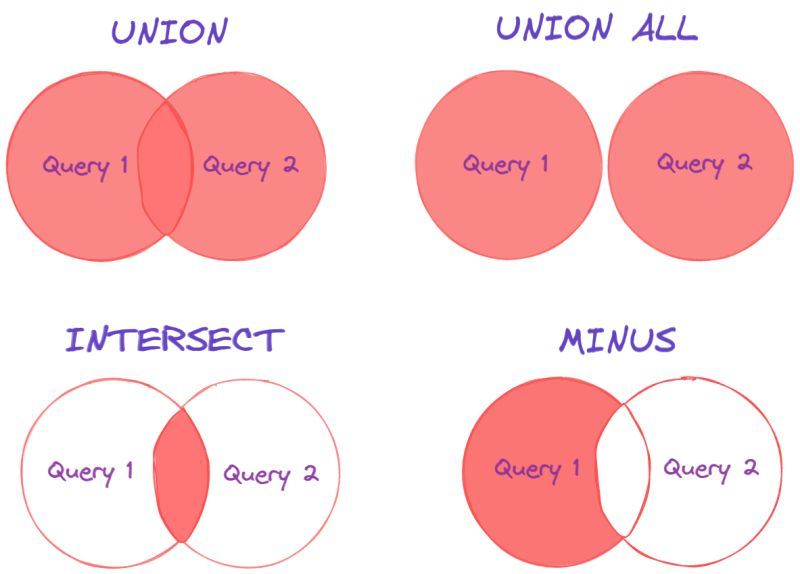
\includegraphics[width=0.4\linewidth]{immagine2.png}
    \end{figure}

    \item \textbf{OPERATORI DELL'ALGEBRA RELAZIONALE:} \begin{itemize}
        \item \textbf{Ridenominazione} $\boldsymbol{\rho}$
        \item \textbf{Selezione} $\boldsymbol{\sigma}$
        \item \textbf{Proiezione} $\boldsymbol{\Pi}$
    \end{itemize}
    \item \textbf{OPERATORE FONDAMENTALE:} JOIN \begin{itemize}
        \item JOIN naturale
        \item Prodotto cartesiano $\times$
        \item Theta-Join
    \end{itemize}
\end{itemize}


\begin{minipage}{.2\textwidth}
  \centering
           \begin{tabular}{|c|c|}
                 \hline
                 \textbf{Padre} & \textbf{Figlio}  \\
                 \hline
                 Adamo & Abele \\
                 \hline
                 Adamo & Caino \\
                 \hline
                 Abramo & Isacco \\
                 \hline
            \end{tabular}
\captionof{table}{Paternità}
\hspace{1em}
\end{minipage}
\hfill
\begin{minipage}{.2\textwidth}
  \centering
           \begin{tabular}{|c|c|}
                 \hline
                 \textbf{Madre} & \textbf{Figlio} \\
                 \hline
                    Eva & Abele \\
                    \hline
                    Eva & Caino \\
                    \hline
                    Sara & Isacco\\
                 \hline
            \end{tabular}
\captionof{table}{Maternità}
\hspace{1em}
\end{minipage}
\hfill
\begin{minipage}{.4\textwidth}
  \centering
           \begin{tabular}{|c|c|}
                 \hline
                 \textbf{Genitore} & \textbf{Figlio} \\
                 \hline
                 Adamo & Abele \\
                 \hline
                 Adamo & Caino \\
                 \hline
                 Abramo & Isacco \\
                 \hline
                    Eva & Abele \\
                    \hline
                    Eva & Caino \\
                    \hline
                    Sara & Isacco\\
                 \hline
            \end{tabular}
\captionof{table}{Unione dopo la ridenominazione}
\hspace{1em}
\end{minipage}

Non posso fare Paternità $\cup$ Maternità perché non sono definite sullo stesso insieme di attributi. Per risolvere il problema uso l'operatore di \textbf{RIDENOMINAZIONE}. 
\Large
\begin{align*}
    \rho_{Genitore \leftarrow Padre} (PATERNITA) \\
    \rho_{Genitore \leftarrow Madre} (MATERNITA)
\end{align*}
\normalsize
 dove $\rho$ è l'operatore e nelle parentesi ci va la relazione.


Quindi ora ho $PATERNITA(Genitore, Figlio)$ e $MATERNITA(Genitore, Figlio)$ e quindi 
\Large
\begin{align*}
    \rho_{Genitore \leftarrow Padre} (PATERNITA) \cup \rho_{Genitore \leftarrow Madre} (MATERNITA)
\end{align*}
\normalsize

\newpage
\subsubsection{Ridenominazione $\rho$}
\begin{itemize}
    \item Operatore unario;
    \item "Modifica lo schema" lasciando inalterata l'istanza;
    \item Permette di cambiare il nome agli attributi, per rendere compatibili domini diversi.
\end{itemize}

\mybox{\textbf{Definizione}
\begin{enumerate}
    \item \textit{Sia $r$ una relazione definita sull'insieme di attributi X e sia Y un altro insieme di attributi con la stessa cardinalità.} Ad esempio:
\begin{align*}
    X = \{Padre, Figlio\}\\Y= \{Genitore,Figlio\}
\end{align*}

\item Siano $A_1,A_2,...A_k$ e $B_1,B_2,...,B_k$ rispettivamente un ordinamento per gli attributi in X e un ordinamento per quelli in Y. 
\item Allora la \textbf{ridenominazione} contiene una tupla $t'$ per ogni tupla $t$ in $r$. $\rho_{B_1,B_2,...,B_k} \leftarrow _{A_1,A_2,...,A_k}(r)$
\end{enumerate}}

Ad esempio, data la tabella $STUDENTE(Matricola, Conome, Nome, Ind, Tel)$, se volessi cambiare solo il numero di telefono scrivo $\rho_{TelPer} \leftarrow _{Tel}(STUDENTE)$. 

Se volessi cambiare tutti gli attributi posso fare $\rho_{\overline{x}'} \leftarrow\overline{x}(STUDENTE)$.

\subsubsection{Selezione $\sigma$}
\begin{itemize}
    \item Operatore unario;
    \item Produce un risultato che ha lo stesso schema dell'operando;
    \item contiene un sottoinsieme delle tuple;
    \item genera una \textit{decomposizione orizzontale}, perché la relazione avrà ancora gli stessi attributi, ma con solo le tuple vere.
    \item il risultato di una selezione è una relazione con lo stesso schema, quindi lo \textbf{stesso} \textbf{grado}, \textbf{cardinalità} $\boldsymbol{\leq}$ di quella di partenza.
\end{itemize}

\mybox{\textbf{Definizione}
Data una relazione $r(x)$, una formula proposizionale $F$ su $x$ \begin{align}
    \sigma_F(r) \to risultato*
\end{align}
 dove $\sigma$ è l'operatore di selezione, $F$ è una formula su $x$ e $r$ è la relazione su cui applico la selezione.
 
 $\to risultato*$: il risultato contiene tutte le tuple di $r$ per cui $F$ è vera. Quindi $F$ descrive la \textit{condizione di selezione.}}

 \textit{Esempio:}\begin{align*}
     STUDENTE(\underline{Matricola}, Cognome, Nome, DataNascita,CittaResidenza,Tel)
 \end{align*}

 \begin{table}[h!]
     \centering
     \begin{tabular}{|c|c|c|c|c|c|}
     \hline
     \textbf{Matricola} & \textbf{Cognome} & \textbf{Nome} & \textbf{DataNascita} & \textbf{CittaResidenza} & \textbf{Tel}\\
     \hline
          VR01 & Rossi & Giulia & 12/12/2005 &  Verona & 347... \\
          \hline
          VR02 & Gialli & Luca & 01/01/2006 &  Milano & 343... \\
          \hline
            VR04 & Gialli & Mario & 03/03/2004 & Verona & 329... \\
          \hline 
     \end{tabular}
     \caption{STUDENTE}
 \end{table}
Se ora io applico l'operazione sotto descritta sulla tabella soprastante
 \begin{align*}
     \sigma_{CittaResidenza = "Verona"}(STUDENTE)
 \end{align*}

 Otterrò il seguente risultato
 
 \begin{table}[h!]
     \centering
     \begin{tabular}{|c|c|c|c|c|c|}
     \hline
     \textbf{Matricola} & \textbf{Cognome} & \textbf{Nome} & \textbf{DataNascita} & \textbf{CittaResidenza} & \textbf{Tel}\\
     \hline
          VR01 & Rossi & Giulia & 12/12/2005 &  Verona & 347... \\
          \hline
            VR04 & Gialli & Mario & 03/03/2004 & Verona & 329... \\
          \hline 
     \end{tabular}
     \caption{STUDENTE dopo l'operazione $\sigma_{CittaResidenza = "Verona"}(STUDENTE)$}
 \end{table}

 \textit{Generalmente il risultato di una selezione è un sottoinseme della relazione su cui viene applicata. Potrebbe essere anche un insieme vuoto o lo stesso insieme, poiché la condizione di selezione potrebbe applicarsi a tutte le tuple presenti in precedenza.}

\mybox{\textbf{Una condizione di selezione può prevedere:}
\begin{itemize}
    \item \textbf{Confronto tra attributo e costante} $A_1 \Theta \hspace{0.3em}costante$ dove $\Theta$ è un operatore $\{=,>,<,...\}$

    \textit{Esempio: }$\sigma_{CittaResidenza = "Verona"}(STUDENTE)$
    \item \textbf{Confronto tra due attributi} $A_1 \Theta A_2$

    \textit{Esempio: }$\sigma_{Cognome = CittaResidenza}(STUDENTE)$
    \item \textbf{Combinazione complessa:} ottenuta combinando condizioni semplici con i connettivi logici. 
       \sitemize{ \item \textbf{AND} $COND_1 \land COND_2$
        \item \textbf{OR} $COND_1 \lor COND_2$
        \item \textbf{NOT} $\lnot COND_1$
   }

    \textit{Esempio:} $\sigma_{Cognome = "Gialli" \land CittaResidenza = "Verona"}(STUDENTE)$
\end{itemize}

}

\textbf{Esempio:}
\begin{table}[h!]
    \centering
    \begin{tabular}{|c|c|c|c|}
        \hline
        \textbf{Matricola} & \textbf{Cognome} & \textbf{Filiale} & \textbf{Stipendio} \\
        \hline
        7309 & Rossi & Roma & 55 \\
        \hline
        5993 & Neri & Milano & 64 \\
        \hline
        9553 & Milano & Milano & 44 \\
        \hline
        5698 & Neri & Napoli & 64 \\
        \hline
    \end{tabular}
    \caption{IMPIEGATO}
\end{table}

\textbf{Effettuare le seguenti query:}
\begin{enumerate}
    \item \textbf{Trovare gli impiegati che guadagnano più di 50:}

    $\sigma_{Stipendio > 50} (IMPIEGATO)$

    Risultato:
    \begin{tabular}{|c|c|c|c|}
            \hline
            \textbf{Matricola} & \textbf{Cognome} & \textbf{Filiale} & \textbf{Stipendio} \\
            \hline
            7309 & Rossi & Roma & 55 \\
            \hline
            5993 & Neri & Milano & 64 \\
            \hline
            5698 & Neri & Napoli & 64 \\
            \hline
        \end{tabular}
    
    \item \textbf{Trovare gli impiegati che guadagnano più di 50 e lavorano a Milano:}

        $\sigma_{Stipendio > 50 \land Filiale = "Milano"} (IMPIEGATO)$
         
         Risultato:
    \begin{tabular}{|c|c|c|c|}
            \hline
            \textbf{Matricola} & \textbf{Cognome} & \textbf{Filiale} & \textbf{Stipendio} \\
            \hline
            5993 & Neri & Milano & 64 \\
        
            \hline
        \end{tabular}
    \item \textbf{Trovare gli impiegati che hanno lo stesso nome della filiale in cui lavorano:}

            $\sigma_{Cognome = Filiale} (IMPIEGATO)$

Risultato:
         \begin{tabular}{|c|c|c|c|}
        \hline
        \textbf{Matricola} & \textbf{Cognome} & \textbf{Filiale} & \textbf{Stipendio} \\
        \hline
 
        9553 & Milano & Milano & 44 \\
        
        \hline
    \end{tabular}
\end{enumerate}

\newpage
\subsubsection{Proiezione $\pi$}
\begin{itemize}
    \item Operatore unario (lavora su una singola relazione)
    \item Produce un risultato che a differenza della selezione \textbf{non ha lo stesso schema dell'operando.}
    \item Il risultato ha lo schema definito su un sottoinsieme degli attributi dello schema dell'operando.
    \item Contiene \textbf{TUTTE le tuple} eliminando i duplicati, effettua una \textbf{decomposizione verticale.}
    \item Tuple uguali collassano in un'unica tupla.
    \item \textbf{Grado} $\boldsymbol{\leq}$ del grado della relazione di partenza.
    \item \textbf{Cardinalità} $\boldsymbol{\leq}$ della cardinalità della relazione di partenza. 
\end{itemize}
Si indica con
    \begin{align*}
        \Pi_{listaAttributi}(OPERANDO)
    \end{align*}
dove $\Pi$ è l'operatore e al pedice ho la lista degli attributi che voglio come risultato e "OPERANDO" è la tabella a cui applico la proiezione.

Ad esempio, facendo $\Pi_{Matricola, Cognome} (IMPIEGATO)$ otterrò:
    \begin{tabular}{|c|c|}
        \hline
        \textbf{Matricola} & \textbf{Cognome} \\
        \hline
        7309 & Rossi \\
        \hline
        5993 & Neri  \\
        \hline
        9553 & Milano \\
        \hline
        5698 & Neri \\
        \hline
    \end{tabular}

Se io scrivessi $\Pi_{Filiale} (IMPIEGATO)$ otterrei: 
    \begin{tabular}{|c|}
        \hline
        \textbf{Filiale} \\
        \hline
        Roma \\
        \hline
        Milano \\
        \hline
        Napoli \\
        \hline
    \end{tabular}
 non ripetendo però la tupla duplicata singleton contenente il valore "Milano".

 \mybox{
 Data la proiezione $\Pi_Y(r)$ il risultato contiene lo stesso numero di tuple di $r$ se e solo se $Y$ è una \textbf{SUPERCHIAVE} di $r$.
\textit{ In generale, quando si effettua una proiezione su una relazione, la cardinalità è certo che rimanga uguale, cioè rimane lo stesso numero di tuple, se e solo se nella lista degli attributi dell'operatore vi è contenuto anche l'attributo (o l'insieme di attributi) chiave}}

\textbf{Possibile domanda d'esame:}
Data una relazione $R_1(\underline{A},B,C,D)$ e la relazione $R_2(\underline{D},\underline{E},F)$ dove $|R_1| = N_1$ e $|R_2| = N_2$. \begin{itemize}
    \item Se effettuo $\Pi_{A} (R_1) \to |\Pi_{A} (R_1)|=N_1$ cioè stessa cardinalità.
    \item Se effettuo $\Pi_{B} (R_1) \to |\Pi_{B} (R_1) | \leq N_1$
    \item Se effettuo $\Pi_{D,E} (R_2) \to | \Pi_{D,E} (R_2) | = N_2$
    \item Se effettuo $\Pi_{D} (R_2) \to | \Pi_{D,E} (R_2) | \leq N_2$
    \item Se effettuo $\sigma_{B = "Verona"} (R_1) \to |\sigma_{B = "Verona"} (R_1) | \leq N_1 $
\end{itemize}

Ad esempio, se volessi trovare matricola e cognome degli impiegati che guadagnano più di 50 scriverò \begin{align*}
    \Pi_{Matricola,Cognome}(\sigma_{Stipendio>50}(IMPIEGATO))
\end{align*}
Otterrò come risultato 
\begin{table}[h!]
    \centering
\begin{tabular}{|c|c|}
        \hline
        \textbf{Matricola} & \textbf{Cognome} \\
        \hline
        7309 & Rossi \\
        \hline
        5993 & Neri  \\
        \hline
        5698 & Neri \\
        \hline
    \end{tabular}
\end{table}

\newpage
\textbf{ESERCIZIO:}

Data la tabella IMPIEGATO seguente:
\begin{table}[h!]
    \centering
    \begin{tabular}{|c|c|c|c|}
        \hline
        \textbf{\underline{Matricola}} & \textbf{Nome} & \textbf{Eta} & \textbf{Stipendio} \\
        \hline
        7309 & Rossi & 34 & 45 \\
        \hline
        5998 & Bianchi & 37 & 38 \\
        \hline
        9553 & Neri & 42 & 35 \\
        \hline
        5698 & Bruni & 43 & 42 \\
        \hline
             4076 & Mori & 45 & 50\\
        \hline
             8123 & Lupi & 46 & 60 \\
        \hline
    \end{tabular}
    \caption{IMPIEGATO}
\end{table}

\textbf{Effetture le seguenti query:}
\begin{enumerate}
    \item \textbf{Trovare la matricola, nome, età e stipendio degli impiegati che guadagnano più di 40:}

    $\sigma_{Stipendio>40}(IMPIEGATO)$

    Risultato: 
    \begin{tabular}{|c|c|c|c|}
        \hline
        \textbf{\underline{Matricola}} & \textbf{Nome} & \textbf{Eta} & \textbf{Stipendio} \\
        \hline
        7309 & Rossi & 34 & 45 \\
        \hline
        5698 & Bruni & 43 & 42 \\
        \hline
             4076 & Mori & 45 & 50\\
        \hline
             8123 & Lupi & 46 & 60 \\
        \hline
    \end{tabular}
    
    Non ho messo la proiezione perché gli attributi che voglio ottenere sono gli stessi della tabella di partenza.
    
    \item \textbf{Trovare matricola, nome ed età degli impiegati che guadagnano più di 40}:

    $\Pi_{Matricola,Nome,Eta}(\sigma_{Stipendio > 40}(IMPIEGATO))$

    Risultato: 
    \begin{tabular}{|c|c|c|}
        \hline
        \textbf{\underline{Matricola}} & \textbf{Nome} & \textbf{Eta}  \\
        \hline
        7309 & Rossi & 34  \\
        \hline
        5698 & Bruni & 43  \\
        \hline
             4076 & Mori & 45 \\
        \hline
             8123 & Lupi & 46  \\
        \hline
    \end{tabular}
    \item \textbf{Trovare nome degli impiegati con un'età minore di 40 che guadagnano più di 40:}

    $\Pi_{Nome}(\sigma_{Eta < 40 \land Stipendio > 40}(IMPIEGATO))$
    
    Risultato: 
    \begin{tabular}{|c|}
        \hline
        \textbf{Nome}  \\
        \hline
        Rossi\\
        \hline
    \end{tabular}
    
\end{enumerate}

Si può indicare anche così:
\begin{center} % ✅ Centra orizzontalmente l'albero
\begin{forest}
for tree={
  draw=none, % ❌ Rimuove i contorni
  rounded corners,
  align=center,
  parent anchor=south,
  child anchor=north,
  l sep=15pt,
  s sep=15pt
}
[{$\pi_{\text{Nome}}$}
  [{$\sigma_{\text{Età} < 40 \land \text{Stipendio} > 40}$}
    [IMPIEGATO]
  ]
]
\end{forest}
\end{center}

\subsubsection{JOIN}
Operatore dell'algebra relazionale che permette di correlare i dati contenuti in relazioni diverse, confrontando i valori. Ne abbiamo due versioni: join naturale e theta-join.

\begin{itemize}
    \item \textbf{Join naturale:} $R_1\bowtie R_2$\sitemize{
    \item Operatore \textbf{binario} (generalizzante)
    \item Correla dati in relazioni diverse sulla base di valori uguali in attributi con lo stesso nome.
    \item Produce un risultato sull'unione degli operandi con tuple costruite ciascuna a partire da una tupla di ciascuno degli operandi combinando le tuple con valori uguali su attributi comuni.
    \item Il \textbf{grado} della relazione ottenuta come risultato del join è minore o uguale (caso del prodotto cartesiano) della somma dei gradi dei due operandi. 
    }

\textbf{Esempio:}

\begin{minipage}{.3\textwidth}
  \centering
    \begin{tabular}{|c|c|}
        \hline
        \textbf{Impiegato} & \textbf{Reparto} \\
        \hline
        Rossi & A \\
        \hline
        Neri &  B \\
        \hline
        Bianchi & B \\
         \hline
        \end{tabular}
  \captionof{table}{R1}
\end{minipage}%
\hfill
\begin{minipage}{.3\textwidth}
  \centering
       \begin{tabular}{|c|c|}
        \hline
        \textbf{Reparto} & \textbf{Capo} \\
        \hline
        A & Mori\\
        \hline
        B & Bruni\\
         \hline
        \end{tabular}
\captionof{table}{R2}
\hspace{1em}
\end{minipage}
\begin{minipage}{.3\textwidth}
  \centering
       \begin{tabular}{|c|c|c|}
        \hline
        \textbf{Impiegato} & \textbf{Reparto} & \textbf{Capo} \\
        \hline
        Rossi & A & Mori\\
        \hline
        Neri & B & Bruni\\
         \hline
         Bianchi & B & Bruni\\
         \hline
        \end{tabular}
\captionof{table}{$R_1\bowtie R_2$}
\hspace{1em}
\end{minipage}
\begin{align*}
    |R_1| = 3; \quad |R_2| = 2; \quad |R_1 \bowtie R_2| = 3.
\end{align*}

\textbf{Dimensione del risultato di un join:} \begin{enumerate}
    \item \textbf{Join completo:} ciascuna tupla dei due operandi contribuisce ad \textit{almeno una} tupla del risultato. Quindi, date le due tabelle di partenza, ogni tupla delle due tabelle di partenza finisce nel risultato. Ad esempio, le tabelle sopra presenti con il loro join rappresentano un \textit{join completo.} La cardinalità del join completo sarà $\geq$ del massimo della cardinalità delle due relazioni: \begin{align*}
        | R_1 \bowtie R_2 | \geq max(|R_1|,|R_2|)
    \end{align*}
    \item \textbf{Join non completo:} alcune tuple (definite \textit{dangling})degli operandi NON contribuiscono al risultato perché non trovano corrispondenza di valore negli attributi comuni nell'altra relazione.

    
\textbf{Esempio:}

\begin{minipage}{.25\textwidth}
  \centering
    \begin{tabular}{|c|c|}
        \hline
        \textbf{Impiegato} & \textbf{Reparto} \\
        \hline
        Rossi & A \\
        \hline
        Neri &  B \\
        \hline
        Bianchi & B \\
         \hline
        \end{tabular}
  \captionof{table}{R1}
\end{minipage}%
\hfill
\begin{minipage}{.25\textwidth}
  \centering
       \begin{tabular}{|c|c|}
        \hline
        \textbf{Reparto} & \textbf{Capo} \\
        \hline
        B & Mori\\
        \hline
        C & Bruni\\
         \hline
        \end{tabular}
\captionof{table}{R2}
\end{minipage}
\hfill
\begin{minipage}{.25\textwidth}
  \centering
       \begin{tabular}{|c|c|c|}
        \hline
        \textbf{Impiegato} & \textbf{Reparto} & \textbf{Capo} \\
        \hline
        Neri & B & Mori\\
         \hline
         Bianchi & B & Mori\\
         \hline
        \end{tabular}
\captionof{table}{$R_1\bowtie R_2$}
\hspace{1em}
\end{minipage}

Non trovo quindi la tupla $\{Rossi,A\}$ e $\{C,Bruni\}$ e $    |R_1| = 3; \quad |R_2| = 2; \quad |R_1 \bowtie R_2| = 2.
$.
\vspace{1em}

La cardinalità massima quindi del join non completo sarà:
\begin{align*}
    |R_1 \bowtie R_2| < |R_1| \times |R_2|
\end{align*}

\item \textbf{Join vuoto:} nessuna tupla degli operandi trova corrispondenza. $|R_1 \bowtie R_2| = 0  $

    
\textbf{Esempio:}

\begin{minipage}{.25\textwidth}
  \centering
    \begin{tabular}{|c|c|}
        \hline
        \textbf{Impiegato} & \textbf{Reparto} \\
        \hline
        Rossi & A \\
        \hline
        Neri &  B \\
        \hline
        Bianchi & B \\
         \hline
        \end{tabular}
  \captionof{table}{R1}
\end{minipage}%
\hfill
\begin{minipage}{.25\textwidth}
  \centering
       \begin{tabular}{|c|c|}
        \hline
        \textbf{Reparto} & \textbf{Capo} \\
        \hline
        D & Mori\\
        \hline
        C & Bruni\\
         \hline
        \end{tabular}
\captionof{table}{R2}
\end{minipage}
\hfill
\begin{minipage}{.25\textwidth}
  \centering
       \begin{tabular}{|c|c|c|}
        \hline
        \textbf{Impiegato} & \textbf{Reparto} & \textbf{Capo} \\
        \hline
        ... & ... & ... \\
         \hline
        \end{tabular}
\captionof{table}{$R_1\bowtie R_2$}
\hspace{1em}
\end{minipage}

In questo caso quindi $|R_1 \bowtie R_2| = 0$.

\item \textit{\textbf{Caso particolare di join completo:}} tutte le tuple di una relazione si combinano con tutte le altre tuple dell'altra relazione.

\textbf{Esempio:}

\begin{minipage}{.25\textwidth}
  \centering
    \begin{tabular}{|c|c|}
        \hline
        \textbf{Impiegato} & \textbf{Reparto} \\
        \hline
        Rossi & F \\
        \hline
        Neri &  F \\
        \hline
        \end{tabular}
  \captionof{table}{R1}
\end{minipage}%
\hfill
\begin{minipage}{.25\textwidth}
  \centering
       \begin{tabular}{|c|c|}
        \hline
        \textbf{Reparto} & \textbf{Capo} \\
        \hline
        F & Mori\\
        \hline
        F & Bruni\\
         \hline
        \end{tabular}
\captionof{table}{R2}
\end{minipage}
\hfill
\begin{minipage}{.25\textwidth}
  \centering
       \begin{tabular}{|c|c|c|}
        \hline
        \textbf{Impiegato} & \textbf{Reparto} & \textbf{Capo} \\
        \hline
        Rossi & F & Mori \\
        \hline
        Rossi & F& Bruni \\
        \hline
        Neri & F & Mori\\
         \hline
         Neri & B & Bruni\\
         \hline
        \end{tabular}
\captionof{table}{$R_1\bowtie R_2$}
\hspace{1em}
\end{minipage}

In questo caso $|R_1 \bowtie R_2| = |R_1| \times |R_2|$. Ogni tupla di $R_1$ è combinabile con ogni tupla di $R_2$.
\end{enumerate}

\mybox{\textbf{Dimensione del risultato del join naturale:}
Il join $R_1\bowtie R_2$ contiene un numero di tuple compreso tra 0 e $|R_1| \times |R_2|$. Quindi $0 \leq |R_1 \bowtie R_2| \leq |R_1| \times |R_2|$.

Inoltre, se il join di $R_1$ e $R_2$ è completo, allora contiene \textit{almeno} un numero di tuple pari al massimo tra la cardinalità di $R_1$ ($|R_1|$) e la cardinalità di $R_2$. ($|R_2|$)
}

\textbf{Considerazioni sui join: }

\mybox{
Date $R_1(A,B)$ e $R_2(B,C)$ in generale $0 \leq |R_1 \bowtie R_2| \leq |R_1| \times |R_2|$. 

\sitemize{
\item  \textbf{Se B è chiave} in $R_2$ allora  $0 \leq |R_1 \bowtie R_2| \leq |R_1|$

\begin{minipage}{.25\textwidth}
  \centering
    \begin{tabular}{|c|c|}
        \hline
        \textbf{A} & \textbf{B} \\
        \hline
        ... & x \\
        \hline
        ... &  x \\
        \hline
        ... &  z \\
        \hline
        \end{tabular}
  \captionof{table}{R1}
\end{minipage}%
\hfill
\begin{minipage}{.25\textwidth}
  \centering
       \begin{tabular}{|c|c|}
        \hline
        \textbf{\underline{B}} & \textbf{C} \\
        \hline
        x & ...\\
        \hline
        y & ...\\
         \hline
        \end{tabular}
\captionof{table}{R2}
\end{minipage}
\hfill
\begin{minipage}{.25\textwidth}
  \centering
       \begin{tabular}{|c|c|c|}
        \hline
        \textbf{A} & \textbf{B} & \textbf{C} \\
        \hline
        ... & x & ... \\
        \hline
        ... & x & ... \\
         \hline
        \end{tabular}
\captionof{table}{$R_1\bowtie R_2$}
\hspace{1em}
\end{minipage}

\item \textbf{Se B è chiave} in $R_2$ \textbf{ed esiste un vincolo di integrità referenziale} tra $R_1.B$ ed $R_2$. 
Allora $|R_1 \bowtie R_2| = |R_1|$.


\begin{minipage}{.25\textwidth}
  \centering
    \begin{tabular}{|c|c|}
        \hline
        \textbf{A} & \textbf{B} \\
        \hline
        ... & x \\
        \hline
        ... &  x \\
        \hline
        ... &  y \\
        \hline
         ... &  \cancel{z} \\
        \hline
        \end{tabular}
  \captionof{table}{R1}
\end{minipage}%
\hfill
\begin{minipage}{.25\textwidth}
  \centering
       \begin{tabular}{|c|c|}
        \hline
        \textbf{\underline{B}} & \textbf{C} \\
        \hline
        x & ...\\
        \hline
        y & ...\\
         \hline
        \end{tabular}
\captionof{table}{R2}
\end{minipage}
\hfill
\begin{minipage}{.25\textwidth}
  \centering
       \begin{tabular}{|c|c|c|}
        \hline
        \textbf{A} & \textbf{B} & \textbf{C} \\
        \hline
        ... & x & ... \\
        \hline
        ... & x & ... \\
         \hline
         ... & y & ... \\
         \hline
        \end{tabular}
\captionof{table}{$R_1\bowtie R_2$}
\hspace{1em}
\end{minipage}


}

}


Se io volessi trovare tutti gli impiegati con l'indicazione del capo, se noto, un join non basterebbe perché vedrei solo le tuple con corrispondenza. Utilizzo quindi un \textbf{JOIN ESTERNO} che estende le tuple anche a quelle che non hanno corrispondenza.

\textbf{JOIN ESTERNO:} 

Prevede che tutte le tuple degli operandi diano un contributo al risultato. Estende con valori NULL le tuple che verrebbero tagliate fuori da un join interno. Abbiamo \textbf{tre versioni del join esterno:} \sitemize{
\item \textbf{Join esterno SINISTRO:} mantiene tutte le tuple del primo operando, estendendole con valori nulli se necessario.

    
\textbf{Esempio:}

\begin{minipage}{.25\textwidth}
  \centering
    \begin{tabular}{|c|c|}
        \hline
        \textbf{Impiegato} & \textbf{Reparto} \\
        \hline
        Rossi & A \\
        \hline
        Neri &  B \\
        \hline
        Bianchi & B \\
         \hline
        \end{tabular}
  \captionof{table}{R1}
\end{minipage}%
\hfill
\begin{minipage}{.25\textwidth}
  \centering
       \begin{tabular}{|c|c|}
        \hline
        \textbf{Reparto} & \textbf{Capo} \\
        \hline
        B & Mori\\
        \hline
        C & Bruni\\
         \hline
        \end{tabular}
\captionof{table}{R2}
\end{minipage}
\hfill
\begin{minipage}{.25\textwidth}
  \centering
       \begin{tabular}{|c|c|c|}
        \hline
        \textbf{Impiegato} & \textbf{Reparto} & \textbf{Capo} \\
        \hline
        Neri & B & Mori\\
         \hline
         Bianchi & B & Mori\\
         \hline
        Rossi & A & NULL\\
         \hline
        \end{tabular}
\captionof{table}{$R_1\bowtie_{LEFT} R_2$}
\hspace{1em}
\end{minipage}

\item \textbf{Join esterno DESTRO:} mantiene tutte le tuple del secondo operando (a destra), estendendole con valori nulli se necessario.


\begin{minipage}{.25\textwidth}
  \centering
    \begin{tabular}{|c|c|}
        \hline
        \textbf{Impiegato} & \textbf{Reparto} \\
        \hline
        Rossi & A \\
        \hline
        Neri &  B \\
        \hline
        Bianchi & B \\
         \hline
        \end{tabular}
  \captionof{table}{R1}
\end{minipage}%
\hfill
\begin{minipage}{.25\textwidth}
  \centering
       \begin{tabular}{|c|c|}
        \hline
        \textbf{Reparto} & \textbf{Capo} \\
        \hline
        B & Mori\\
        \hline
        C & Bruni\\
         \hline
        \end{tabular}
\captionof{table}{R2}
\end{minipage}
\hfill
\begin{minipage}{.25\textwidth}
  \centering
       \begin{tabular}{|c|c|c|}
        \hline
        \textbf{Impiegato} & \textbf{Reparto} & \textbf{Capo} \\
        \hline
        Neri & B & Mori\\
         \hline
         Bianchi & B & Mori\\
         \hline
        NULL & C & Bruni\\
         \hline
        \end{tabular}
\captionof{table}{$R_1\bowtie_{RIGHT} R_2$}
\hspace{1em}
\end{minipage}


\item \textbf{Join esterno COMPLETO:} mantiene tutte le tuple di entrambi gli operandi, estendendole con valori nulli se necessario.

\begin{minipage}{.25\textwidth}
  \centering
    \begin{tabular}{|c|c|}
        \hline
        \textbf{Impiegato} & \textbf{Reparto} \\
        \hline
        Rossi & A \\
        \hline
        Neri &  B \\
        \hline
        Bianchi & B \\
         \hline
        \end{tabular}
  \captionof{table}{R1}
\end{minipage}%
\hfill
\begin{minipage}{.25\textwidth}
  \centering
       \begin{tabular}{|c|c|}
        \hline
        \textbf{Reparto} & \textbf{Capo} \\
        \hline
        B & Mori\\
        \hline
        C & Bruni\\
         \hline
        \end{tabular}
\captionof{table}{R2}
\end{minipage}
\hfill
\begin{minipage}{.25\textwidth}
  \centering
       \begin{tabular}{|c|c|c|}
        \hline
        \textbf{Impiegato} & \textbf{Reparto} & \textbf{Capo} \\
        \hline
        Rossi & A & NULL\\
        \hline
        Neri & B & Mori\\
         \hline
         Bianchi & B & Mori\\
         \hline
        NULL & C & Bruni\\
         \hline
        \end{tabular}
\captionof{table}{$R_1\bowtie_{FULL} R_2$}
\hspace{1em}
\end{minipage}
}

\newpage
\item \textbf{Join naturale N-ario:}

\textbf{Proprietà del join naturale:} (alcuni non valgono per i join esterni) 

\sitemize{
\item Il join naturale è \textbf{commutativo}. Non lo è il left/right-join, mentre il full join sì.
\item Il join naturale è \textbf{associativo}. Cioè $R_1 \bowtie (R_2 \bowtie R_3) = (R_1 \bowtie R_2) \bowtie R_3 = R_1 \bowtie R_2 \bowtie R_3$

\textbf{Esempio:} dato lo schema \begin{align*}
    IMPIEGATO(NomeImpiegato, NomeReparto) \\
    REPARTO(NomeReparto, NomeCapo) \\
    CAPOPROGETTO(NomeCapo, NomeProgetto) \\
    PROGETTO(NomeProgetto, Descrizione)
\end{align*}
Allora $IMPIEGATO \bowtie REPARTO \bowtie CAPOPROGETTO \bowtie PROGETTO$ avrà come schema:
\begin{align*}
    RIS(NomeImpiegato,NomeReparto,NomeCapo,NomeProgetto,Descrizione)
\end{align*}
}

\mybox{


\textbf{ATTENZIONE:} dati $R_1(X_1) \bowtie R_2(X_2)$ fin'ora abbiamo visto che $| X_1 \cap X_2| > 0 $, e nel nostro caso degli esempi $X_1 \cap X_2 = \{B\}$. 

Abbiamo due \textbf{casi} \textbf{estremi}: \sitemize{
\item $X_1 = X_2$. Allora $R_1 \bowtie R_2 \equiv R_1 \cap R_2$ 

\textit{Esempio:} $R_1(A,B) \bowtie R_2(A,B)$

\begin{minipage}{.25\textwidth}
  \centering
    \begin{tabular}{|c|c|}
        \hline
        \textbf{A} & \textbf{B} \\
        \hline
        1 & x \\
        \hline
        2 &  x \\
        \hline
        3 & z \\
         \hline
        \end{tabular}
  \captionof{table}{R1}
\end{minipage}%
\hfill
\begin{minipage}{.25\textwidth}
  \centering
         \begin{tabular}{|c|c|}
        \hline
        \textbf{A} & \textbf{B} \\
        \hline
        1 & x\\
        \hline
        2 & z\\
         \hline
         3 & z \\
         \hline
        \end{tabular}
\captionof{table}{R2}
\end{minipage}
\hfill
\begin{minipage}{.25\textwidth}
  \centering
       \begin{tabular}{|c|c|}
        \hline
        \textbf{A} & \textbf{B} \\
        \hline
        1 & x \\
        \hline
        3 & z \\
         \hline
        \end{tabular}
\captionof{table}{$R_1\bowtie R_2$}
\hspace{1em}
\end{minipage}



\item $X_1 \cap X_2 = \emptyset$. Allora $R_1 \bowtie R_2 \equiv R_1 \times R_2$

Poiché $X_1$ e $X_2$ NON hanno attributi in comune, la condizione che le due tuple devono avere gli stessi valori sugli attributi comuni degenera in una condizione sempre verificata. Quindi il risultato contiene tutte le tuple ottenute dalla combinazione in tutti i modi possibili delle tuple degli operandi. 

\textit{Esempio:} $R_1(A,B) \bowtie R_2(C,D)$

\begin{minipage}{.25\textwidth}
  \centering
    \begin{tabular}{|c|c|}
        \hline
        \textbf{A} & \textbf{B} \\
        \hline
        1 & x \\
        \hline
        2 &  x \\
        \hline
        3 & z \\
         \hline
        \end{tabular}
  \captionof{table}{R1}
\end{minipage}%
\hfill
\begin{minipage}{.25\textwidth}
  \centering
       \begin{tabular}{|c|c|}
        \hline
        \textbf{C} & \textbf{D} \\
        \hline
        a & 3\\
        \hline
        x & 4\\
         \hline
         w & 5 \\
         \hline
        \end{tabular}
\captionof{table}{R2}
\end{minipage}
\hfill
\begin{minipage}{.25\textwidth}
  \centering
\begin{tabular}{|c|c|c|c|}
        \hline
        \textbf{A} & \textbf{B} & \textbf{C} & \textbf{D} \\
        \hline
        1 & x & a & 3 \\
        \hline
        1 & x & x & 4 \\
        \hline
        1 & x & w & 5 \\
        \hline
        2 & x & a & 3 \\
        \hline
        2 & x & x & 4 \\
        \hline
        2 & x & w & 5 \\
        \hline
        3 & z & a & 3 \\
        \hline
        3 & z & x & 4 \\
        \hline
        3 & z & w & 5 \\
        \hline
    \end{tabular}
\captionof{table}{$R_1\bowtie R_2$}
\hspace{1em}
\end{minipage}


Un join naturale su relazioni che non hanno attributi in comune è un \textbf{prodotto cartesiano}. Il risultato contiene sempre un numero di tuple pari al prodotto della cardinalità dei due. $|R_1 \bowtie R_2| = |R_1| \times |R_2|$

}
}


\item \textbf{Prodotto cartesiano $R_1\times R_2$:} il risultato di $R_1(X_1) \bowtie R_2(X_2)$ con $X_1 \cap R_2 = \emptyset$ è una tabella con schema formato da tutti gli attributi di $X_1$ e $X_2$, il cui $grado (R_1 \times R_2) = grado(R_1) + grado(R_2)$. 

L'istanza, invece, è formata da \textit{tutte le possibile coppie di tuple} di $R_1$ e $R_2$. Quindi 
$|R_1 \bowtie R_2| = |R_1| \times |R_2|$

\newpage
\textbf{Esempio:} in questo esempio avviene un prodotto cartesiano perché, anche se Reparto e Codice indicano la stessa cosa, non posseggono lo stesso nome dell'attributo. Questa condizione viene risolta nel seguente punto col \textit{theta-join} (vedi punto elenco successivo).

\noindent \begin{minipage}{.25\textwidth}
  \centering
    \begin{tabular}{|c|c|}
        \hline
        \textbf{Impiegato} & \textbf{Reparto} \\
        \hline
        Rossi & A \\
        \hline
        Neri &  B \\
        \hline
        Bianchi & B \\
         \hline
        \end{tabular}
  \captionof{table}{IMPIEGATO}
\end{minipage}%
\hspace{0.1em}
\begin{minipage}{.25\textwidth}
  \centering
       \begin{tabular}{|c|c|}
        \hline
        \textbf{Codice} & \textbf{Capo} \\
        \hline
        A & Mori\\
        \hline
        B & Bruni\\
         \hline
        \end{tabular}
\captionof{table}{REPARTO}
\end{minipage}
\hspace{0.1em}
\begin{minipage}{.5\textwidth}
  \centering
    \begin{tabular}{|c|c|c|c|}
        \hline
        \textbf{Impiegato} & \textbf{Reparto} & \textbf{Codice} & \textbf{Capo} \\
        \hline
        Rossi & A & A & Mori \\
        \hline
        Rossi & A & B & Bruni \\
        \hline
        Neri & B & A & Mori \\
        \hline
        Neri & B & B & Bruni \\
        \hline
        Bianchi & B & A & Mori \\
        \hline
        Bianchi & B & B & Bruni \\
        \hline
    \end{tabular}
  \captionof{table}{IMPIEGATO $\bowtie$ REPARTO\newline
  (o meglio IMPIEGATO $\times$ REPARTO)}
\end{minipage}




\item \textbf{Theta-join:} operatore definito come\textbf{ prodotto cartesiano seguito da una selezione}. 

Data la formula proposizionale $F$ (congiunzione \emph{AND} di atomi di confronto, cioè F può essere $A=B, A > B, A < B, etc...$) e due relazioni $R_1(X_1)$ e $R_2(X_2)$ con $X_1 \cap X_2 = \emptyset$, si definisce 

\textbf{Theta-join:} \begin{align*}
    R_1 \bowtie_F R_2 = \sigma_F(R_1\bowtie R_2)
\end{align*}

\end{itemize}

\textbf{Esempio:}
\begin{align*}
    \sigma_{Reparto =Codice} (IMPIEGATO \bowtie REPARTO) = IMPIEGATO \bowtie_{Reparto = Codice}REPARTO
\end{align*}


\noindent \begin{minipage}{.25\textwidth}
  \centering
    \begin{tabular}{|c|c|}
        \hline
        \textbf{Impiegato} & \textbf{Reparto} \\
        \hline
        Rossi & A \\
        \hline
        Neri &  B \\
        \hline
        Bianchi & B \\
         \hline
        \end{tabular}
  \captionof{table}{IMPIEGATO}
\end{minipage}%
\hspace{1em}
\begin{minipage}{.25\textwidth}
  \centering
       \begin{tabular}{|c|c|}
        \hline
        \textbf{Reparto} & \textbf{Capo} \\
        \hline
        A & Mori\\
        \hline
        B & Bruni\\
         \hline
        \end{tabular}
\captionof{table}{REPARTO}
\end{minipage}
\hspace{0.1em}
\begin{minipage}{.5\textwidth}
  \centering
       \begin{tabular}{|c|c|c|}
        \hline
        \textbf{Impiegato} & \textbf{Reparto} & \textbf{Capo} \\
        \hline
        Rossi & A & Mori\\
         \hline
         Neri & B & Bruni\\
         \hline
         Bianchi & B & Bruni \\
         \hline
        \end{tabular}
\captionof{table}{$IMPIEGATO\bowtie_{Reparto = Codice} REPARTO$}
\end{minipage}
\vspace{1em}
\noindent\hrule
\vspace{1em}
\textbf{Esempio$^2$:} dato il seguente schema
\begin{align*}
    IMPIEGATO(\underline{Matricola}, Nome, Eta, Stipendio) \\
    SUPERVISIONE(\underline{Impiegato},Capo)
\end{align*}
\mybox{\textbf{Osservazione:}
Scrivere
\begin{align*}
    IMPIEGATO(\underline{Matricola}, Nome, Eta, Stipendio) \\
    SUPERVISIONE^1(\underline{Impiegato},Capo)
\end{align*}

è molto diverso da scrivere
\begin{align*}
    IMPIEGATO(\underline{Matricola}, Nome, Eta, Stipendio) \\
    SUPERVISIONE^2(\underline{Impiegato}, \underline{Capo})
\end{align*}

Poiché $SUPERVISIONE^1$ permette una relazione 1-N tra impiegato e capo, mentre $SUPERVISIONE^2$ permette una relazione N-N tra impiegato e capo. \small{\textit{(verrà approfondito in seguito)}} \normalsize
\sitemize{
\item Cioè, $SUPERVISIONE^1$ permette che per ogni impiegato vi sia \emph{uno ed un solo} capo, infatti, la tupla che contiene lo stesso impiegato non si può ripetere; dunque, un impiegato in questo schema non può avere due capi. 

\item Se invece specifico $SUPERVISIONE^2$, sto permettendo che ogni impiegato abbia \emph{almeno uno o più} capi e che, quindi, ciascun capo abbia almeno uno o più impiegati. Infatti, la condizione di super-chiave è sulla coppia Impiegato-Capo. Non potrò ripetere due volte che lo stesso impiegato ha lo stesso capo (ad esempio dire "A è impiegato di B e A è impiegato di B"), ma invece potrò dire che lo stesso impiegato ha più capi (ad esempio, "A è impiegato di B e A è impiegato di C e D è impiegato di B"). 
}


}

\textbf{Esercizio:}
\textit{Trovare le matricole dei capi degli impiegati che guadagnano più di 40}
\vspace{1em}

\begin{minipage}{.5\textwidth}
  \centering
\begin{tabular}{|c|c|c|c|}
        \hline
        \textbf{\underline{Matricola}} & \textbf{Nome} & \textbf{Eta} & \textbf{Stipendio} \\
        \hline
        7309 & Rossi & 34 & 45 \\
        \hline
        5998 & Bianchi & 37 & 38 \\
        \hline
        9553 & Neri & 42 & 35 \\
        \hline
        5698 & Bruni & 43 & 42 \\
        \hline
             4076 & Mori & 45 & 50\\
        \hline
             8123 & Lupi & 46 & 60 \\
        \hline
    \end{tabular}
\captionof{table}{IMPIEGATO}
\end{minipage}
\begin{minipage}{.5\textwidth}
  \centering
        \begin{tabular}{|c|c|}
        \hline
        \textbf{Impiegato} & \textbf{Capo}\\
        \hline
         7309 & 5698 \\
         \hline
         5998 & 5698 \\
         \hline
    \end{tabular}
\captionof{table}{SUPERVISIONE}
\end{minipage}

\textbf{Soluzione:}
\begin{align*}
    \Pi_{Capo}(SUPERVISIONE \bowtie_{Impiegato = Matricola }(\sigma_{Stipendio>40}(IMPIEGATO)))
\end{align*}

\textbf{Rappresentazione ad albero della soluzione:}

\begin{center}
    \begin{forest}
for tree={
    align=center,
    parent anchor=south,
    child anchor=north,
    l sep=10pt,
    s sep=15pt,
    font=\sffamily,
}
[
    $\pi_{\text{Capo}}$
    [
        $\bowtie_{\text{Impiegato} = \text{Matricola}}$
        [SUPERVISIONE]
        [
            $\sigma_{\text{Stipendio} > 40}$
            [IMPIEGATO]
        ]
    ]
]
\end{forest}
\end{center}

\subsection{Rappresentazione delle espressioni tramite gli alberi}
Ogni espressione dell'algebra relazionale si può rappresentare mediante un albero sintattico che esprime l'ordine di valutazione degli operatori.

\textbf{Esempi usando un paio di query difficili:}

\textit{Trovare gli impiegati che guadagnano più del proprio capo, mostrando nel risultato Matricola, Nome e stipendio dell'impiegato e del capo.}

\vspace{1em}
\begin{minipage}{0.5\textwidth}
\centering
    \begin{tabular}{|c|c|c|c|}
        \hline
        \textbf{\underline{Matricola}} & \textbf{Nome} & \textbf{Eta} & \textbf{Stipendio} \\
        \hline
        7309 & Rossi & 34 & 45 \\
        \hline
        5998 & Bianchi & 37 & 38 \\
        \hline
        9553 & Neri & 42 & 35 \\
        \hline
        5698 & Bruni & 43 & 42 \\
        \hline
             4076 & Mori & 45 & 50\\
        \hline
             8123 & Lupi & 46 & 60 \\
        \hline
    \end{tabular}
    \captionof{table}{IMPIEGATO}
\end{minipage}
\begin{minipage}{0.5\textwidth}
\centering
    \begin{tabular}{|c|c|}
        \hline
        \textbf{Impiegato} & \textbf{Capo}\\
        \hline
         7309 & 5698 \\
         \hline
         5998 & 5698 \\
         \hline
         9553 & 4076 \\
        \hline
        5698 & 4076 \\
        \hline
        4076 & 8123 \\
        \hline
    \end{tabular}
    \captionof{table}{SUPERVISIONE}
\end{minipage}

\textbf{Soluzione con albero:}
\large

\begin{center}
    \begin{forest}
for tree={
    align=center,
    parent anchor=south,
    child anchor=north,
    l sep=10pt,
    s sep=15pt,
    font=\sffamily,
}
[
    $\Pi_{\text{MatrC,NomeC,StpC,Matricola,Nome,Stipendio}}$
    [
        $\sigma_{\text{Stipendio} > \text{StpC}}$
        [
            $\bowtie_{\text{Matricola} = \text{Capo}}$
            [
                $\rho_{\substack{\text{MatrC,NomeC,EtaC,StpC} \\ \leftarrow \text{Matricola,Nome,Eta,Stipendio}}}$
                [IMPIEGATO]
            ]
            [
                $\bowtie_{\text{Impiegato} = \text{Matricola}}$
                [SUPERVISIONE]
                [IMPIEGATO]
            ]
        ]
    ]
]
\end{forest}
\end{center}

\newpage
\textbf{Soluzione in algebra relazionale:}

\begin{align*}
    \Pi_{MatrC,NomeC,StpC,Matricola,Nome, Stipendio}(  \qquad \qquad\qquad\qquad\qquad\qquad\qquad\qquad \qquad\\
    \sigma_{Stipendio > StpC}( \qquad\qquad\qquad\qquad\qquad\qquad\qquad\qquad\qquad\qquad\qquad\qquad\qquad\\
    \rho_{MatrC,NomeC,EtaC,StpC \leftarrow Matricola, Nome, Eta, Stipendio} (IMPIEGATO)\qquad\qquad \\ \bowtie_{Matricola = Capo}(\qquad\qquad\qquad\qquad\qquad\qquad\qquad\qquad\qquad\qquad\qquad\\SUPERVISIONE \bowtie_{Impiegato = Matricola} IMPIEGATO)))
\end{align*}


\normalsize
\textbf{Query 2:} Trovare le matricole dei capi i cui impiegati guadagnano \emph{TUTTI} più di 40. 

\textit{Qua la soluzione si affida all'insiemistica, ovvero al sottrarre dall'insieme di tutti i capi quelli che hanno impiegati che guadagnano meno o uguale di 40.} 

\textbf{Soluzione in algebra relazionale:}
\begin{align*}
    \Pi_{Capo}(SUPERVISIONE) -\Pi_{Capo} (SUPERVISIONE\bowtie_{Impiegato = Matricola}(\sigma_{Stipendio \leq40}(IMPIEGATO) ))
\end{align*}
\textbf{Soluzione in albero:}

\begin{center}
\begin{forest}
for tree={
    % draw, % senza bordi
    align=center,
    parent anchor=south,
    child anchor=north,
    l sep=10pt,
    s sep=15pt,
    edge={->},
    rounded corners,
    font=\sffamily,
}
[
    $-$
    [
        $\Pi_{\text{Capo}}$
        [SUPERVISIONE]
    ]
    [
        $\Pi_{\text{Capo}}$
        [
            $\bowtie_{\text{Impiegato} = \text{Matricola}}$
            [SUPERVISIONE]
            [
                $\sigma_{\text{Stipendio} \leq 40}$
                [IMPIEGATO]
            ]
        ]
    ]
]
\end{forest}
\end{center}

\subsection{Equivalenza di espressioni algebriche}
\textbf{Equivalenza:} due espressioni in algebra relazionale sono equivalenti se producono lo stesso risultato. Cioè \begin{align*}
    X\times(Y + Z) \equiv X \times Y + X\times Z
\end{align*}

In algebra relazionale abbiamo due tipi di equivalenza:
\begin{itemize}
    \item Equivalenza \textbf{assoluta:} \begin{align*}
        \Pi_{A,B}(\sigma_{A>0}(R)) \equiv \sigma_{A>0} (\Pi_{A,B}(R))
    \end{align*}
    \item Equivalenza che \textbf{dipende dallo schema:} \begin{align*}
        \Pi_{A,B} (R_1) \bowtie \Pi_{A,C}(R_2) \equiv_R \Pi_{A,B,C}(R_1 \bowtie R_2)
    \end{align*} che vale solo se nello schema R l'intersezione tra gli attributi di $R_1$ e $R_2$ è pari ad $A$.
\end{itemize}

\mybox{\textbf{A cosa servono le equivalenze tra espressioni algebriche?}

Le espressioni equivalenti servono ai DBMS per ottimizzare le query che poniamo, affinché si trovino quelle meno costose computazionalmente, ovvero quelle che si portano dietro meno tuple.
Sono interessanti le trasformazioni di equivalenze che riducono le dimensioni dei risultati intermedi.
}

\newpage
\subsection{Trasformazioni di equivalenza} 
\begin{itemize}
    \item \textbf{Anticipazione delle selezioni rispetto al join} (PUSHING SELECTIONS DOWN): \begin{align*}
        \sigma_F(R_1\bowtie R_2) \equiv R_1\bowtie \sigma_F(R_2)
    \end{align*}
    se la condizione F fa riferimento solo ad attributi di $R_2$.
    
    Nella rappresentazione ad albero si rappresenta così:
\begin{center}
    \begin{forest}
for tree={
    align=center,
    parent anchor=south,
    child anchor=north,
    l sep=10pt,
    s sep=15pt,
    font=\sffamily,
}
[
    $\sigma_{F}$
    [
        $\bowtie$
        [${R_1}$]
        [${R_2}$]
    ]
]
\end{forest} $\quad\leftarrow$ equivale a 
$\rightarrow\quad$
\begin{forest}
for tree={
    align=center,
    parent anchor=south,
    child anchor=north,
    l sep=10pt,
    s sep=15pt,
    font=\sffamily,
}
[
    $\bowtie$
    [${R_1}$]
    [
        $\sigma_{F}$
        [${R_2}$]
    ]
]
\end{forest}
\end{center}

    \item \textbf{Anticipazione della proiezione rispetto al join} (PUSHING PROJECTIONS DOWN)\begin{align*}
        \Pi_{X_1,Y_2}(R_1 \bowtie R_2) \equiv R_1 \bowtie \Pi_{Y_2}(R_2)
    \end{align*}
    con $Y_2 \subseteq X_2$ e $Y_2 \supseteq (X_1 \cap X_2)$
    \begin{center}
        \begin{forest}
  for tree={
    align=center,
    parent anchor=south,
    child anchor=north,
    l sep=15pt
  }
  [$\Pi_{X_1,Y_2}$
    [$\bowtie$
      [{$R_1$}]
      [{$R_2$}]
    ]
  ]
\end{forest}
$\quad\leftarrow$ equivale a $\rightarrow\quad$ \begin{forest}
  for tree={
    align=center,
    parent anchor=south,
    child anchor=north,
    l sep=15pt
  }
  [$\bowtie$
    [{$R_1$}]
    [$\Pi_{Y_2}$
      [{$R_2$}]
    ]
  ]
\end{forest}
    \end{center}
    \textit{La strategia in tutti questi casi è che se non mi serve quello che non appare nel risultato e quello che non è coinvolto nel join, allora lo rimuovo agli inizi della query.}
    \item \textbf{Atomizzazione delle selezioni:} \begin{align*}
        \sigma_{F_1 \land F_2} (R) \equiv \sigma_{F_1}(\sigma_{F_2}(R))
    \end{align*}
    \begin{center}
    \begin{forest}
      for tree={
        align=center,
        parent anchor=south,
        child anchor=north,
        l sep=15pt
      }
      [$\sigma_{F_1 \land F_2}$
        [{$R$}]
      ]
    \end{forest}
    $\quad\leftarrow$ equivale a $\rightarrow\quad$
    \begin{forest}
      for tree={
        align=center,
        parent anchor=south,
        child anchor=north,
        l sep=15pt
      }
      [$\sigma_{F_1}$
        [$\sigma_{F_2}$
          [{$R$}]
        ]
      ]
    \end{forest}
\end{center}

\item \textbf{Idempotenza delle proiezioni:} data una generica espressione algebrica $E$ \begin{align*}
    \Pi_X(E) \equiv \Pi_X(\Pi_{X_,Y} (E))
\end{align*}

\item \textbf{Distributività della selezione rispetto all'unione:} \begin{align*}
    \sigma_F(R_1 \cup R_2) \equiv \sigma_F(R_1) \cup \sigma_F(R_2)
\end{align*}

\item \textbf{Distributività della proiezione rispetto all'unione:} \begin{align*}
\Pi_X(R_1 \cup R_2) \equiv \Pi_X(R_1) \cup \Pi_X(R_2)\end{align*}
\end{itemize}
\mybox{\textbf{Trasformazioni di equivalenza:}
lo scopo delle trasformazioni di equivalenza è quello di anticipare \textit{il prima possibile} la \emph{proiezione e selezione} all'interno di un'espressione algebrica (o interrogazione) così da ottimizzarne le prestazioni. Le prestazioni vengono ottimizzate perché anticipando queste due operazioni si "scremano", cioè si escludono, presto le colonne o le tuple che non non interessano alla risoluzione dell'interrogazione, così da ridurre il carico a tutte le operazioni che seguiranno. }


\textbf{Esempio:} dato lo schema \begin{align*}
    IMPIEGATO(\underline{Matricola}, Nome, Eta, Stipendio) \\
    SUPERVISIONE (\underline{Impiegato}, Capo)
\end{align*}

E data la seguente query che richiede i capi che hanno impiegati minori di 30 anni:
 \begin{align*}
     \Pi_{Capo}(\sigma_{Matricola = Impiegato \land Eta <30}(IMPIEGATO \bowtie SUPERVISIONE) )
 \end{align*}
è equivalente alla seguente query
\begin{align*}
    \Pi_{Capo}(\Pi_{Matricola}(\sigma_{Eta < 30}(IMPIEGATO)) \bowtie_{Matricola = Impiegato} SUPERVISIONE)
\end{align*}

\subsection{Algebra con valori nulli}
Dato lo schema seguente
\begin{table}[h!]
    \centering
 \begin{tabular}{|c|c|c|c|}
            \hline
            \textbf{Matricola} & \textbf{Cognome} & \textbf{Filiale} & \textbf{Eta} \\
            \hline
            7309 & Rossi & Roma & 32 \\
            \hline
            5998 & Neri & Milano & 45 \\
            \hline
            9553 & Bruni & Milano & NULL \\
            \hline
        \end{tabular}
\end{table}

\sitemize{\item Se io effettuo la query $\sigma_{Eta > 40} (IMPIEGATO)$ il risultato darà solo Neri.

\item Mentre se effettuo la query $\sigma_{Eta \leq 40} (IMPIEGATO)$ il risultato darà solo Rossi
}
Come si può notare, quindi, purtroppo l'unione delle due espressioni algebriche non ci dà la totalità delle tuple della tabella. Dovremo includere la seguente espressione: \begin{align*}
    \sigma_{Eta \ IS\ NULL}(IMPIEGATO)
\end{align*}

Quindi: \begin{align*}
    \sigma_{Eta >40} (IMPIEGATO) \cup \sigma_{Eta \leq 40} (IMPIEGATO) \cup \sigma_{Eta\ IS\ NULL} (IMPIEGATO) = IMPIEGATO
\end{align*}


\textbf{Esercizi:}
dato il seguente schema
\begin{align*}
    STUDENTE(\underline{Matricola}, Cognome, Nome, DataNascita) \\
    ESAME(\underline{MatrStud} \to STUDENTE.Matricola,\underline{CodIns} \to INSEGNAMENTO.Codice, Voto, Data) \\
    INSEGNAMENTO(\underline{Codice},Titolo, CFDoc \to DOCENTE.CF, AA)\\
    DOCENTE(\underline{CF}, Cognome, Nome, DataNascita) \\
\end{align*}
\begin{enumerate}
    \item \textbf{Trovare cognome, nome e data di nascita di docenti e studenti.}
    \begin{align*}
        \Pi_{Cognome,Nome, DataN} (STUDENTE) \cup \Pi_{Cognome,Nome, DataN} (STUDENTE) 
    \end{align*}
    \begin{center}
    \begin{forest}
      for tree={
        align=center,
        parent anchor=south,
        child anchor=north,
        l sep=15pt
      }
      [$\cup$
        [$\Pi_{\text{Cognome, Nome, DataN}}$
          [STUDENTE]
        ]
        [$\Pi_{\text{Cognome, Nome, DataN}}$
          [STUDENTE]
        ]
      ]
    \end{forest}
\end{center}

    
    \item \textbf{Trovare cognome nome degli studenti nati nel 2005}
    
    \begin{align*}
        \Pi_{Cognome, Nome}(\sigma_{DataN \geq 2005/01/01}(\sigma_{DataN < 2006/01/01}(STUDENTE)))
    \end{align*}
    oppure 
    \begin{align*}
        \Pi_{Cognome, Nome}(\sigma_{DataN \geq 2005/01/01 \land DataN < 2006/01/01}(STUDENTE))
    \end{align*}

    \begin{center}
    \begin{forest}
      for tree={
        align=center,
        parent anchor=south,
        child anchor=north,
        l sep=15pt
      }
      [$\Pi_{\text{Cognome, Nome}}$
        [$\sigma_{\text{DataN} \geq \text{2005/01/01} \land\ \text{DataN} < \text{2006/01/01}}$
          [STUDENTE]
        ]
      ]
    \end{forest}
\end{center}


    \item \textbf{Trovare cognome e nome degli studenti che NON sono nati nel 2005.}

    Ci sono diverse soluzioni:
questa non va bene, devi fare prima sottrazione e poi proiezione
    \begin{align*}
        \Pi_{Cognome,Nome}(STUDENTE - \sigma_{DataN \geq 2005/01/01}(\sigma_{DataN < 2006/01/01}(STUDENTE)))
    \end{align*}

    \begin{center}
    \begin{forest}
      for tree={
        align=center,
        parent anchor=south,
        child anchor=north,
        l sep=15pt
      }
      [$\Pi_{\text{Cognome, Nome}}$
        [$-$
          [STUDENTE]
          [$\sigma_{\text{DataN} \geq \text{2005/01/01}}$
            [$\sigma_{\text{DataN} < \text{2006/01/01}}$
              [STUDENTE]
            ]
          ]
        ]
      ]
    \end{forest}
\end{center}
   \mybox{\textbf{ATTENZIONE:}
   Se scrivessi la seguente espressione, invece, che inverte ordine di proiezione e sottrazione \begin{align*}
        \Pi_{Cognome,Nome}(STUDENTE) - \Pi_{Cognome, Nome}(\sigma_{DataN \geq 2005/01/01}(\sigma_{DataN < 2006/01/01}(STUDENTE)))
   \end{align*}
   Questo mi escluderebbe casi di omonimia. Ad esempio, se ci fosse una "Sara Rossi" nata nel 2008 e una "Sara Rossi" nata nel 2005, la sottrazione impedirebbe di vedere quella nata nel 2008.
   }
    oppure un'altra soluzione è:
        \begin{align*}
            \Pi_{Cognome, Nome}(\sigma_{DataN < 2005/01/01 \lor DataN \geq 2006/01/01}(STUDENTE))
        \end{align*}

        \begin{center}
    \begin{forest}
      for tree={
        align=center,
        parent anchor=south,
        child anchor=north,
        l sep=15pt
      }
      [$\Pi_{\text{Cognome, Nome}}$
        [$\sigma_{\text{DataN} < \text{2005/01/01} \lor\ \text{DataN} \geq \text{2006/01/01}}$
          [STUDENTE]
        ]
      ]
    \end{forest}
\end{center}
    oppure 
    \begin{align*}
        \Pi_{Cognome, Nome}(\sigma_{DataN < 2005/01/01}(STUDENTE)) \cup \Pi_{Cognome, Nome}(\sigma_{DataN \geq 2006/01/01}(STUDENTE)) 
    \end{align*}
    \begin{center}
    \begin{forest}
      for tree={
        align=center,
        parent anchor=south,
        child anchor=north,
        l sep=15pt
      }
      [$\cup$
        [$\Pi_{\text{Cognome, Nome}}$
          [$\sigma_{\text{DataN} < \text{2005/01/01}}$
            [STUDENTE]
          ]
        ]
        [$\Pi_{\text{Cognome, Nome}}$
          [$\sigma_{\text{DataN} \geq \text{2006/01/01}}$
            [STUDENTE]
          ]
        ]
      ]
    \end{forest}
\end{center}
\item \textbf{Trovare cognome e nome dei docenti che hanno tenuto il corso di Basi di Dati nell'A.A. 2020/2021}
\begin{align*}
    \Pi_{Nome,Cognome}(DOCENTE \bowtie_{CF = CF}\Pi_{CFDoc}((\sigma_{Titolo =" Basi\ di\  dati"\ \land AA=2020/2021}(INSEGNAMENTO)))
\end{align*}
\begin{center}
\begin{forest}
  for tree={
    align=center,
    parent anchor=south,
    child anchor=north,
    l sep=15pt
  }
  [$\Pi_{\text{Nome, Cognome}}$
    [$\bowtie_{\text{CF} = \text{CFDoc}}$
      [DOCENTE]
      [$\Pi_{\text{CFDoc}}$
        [$\sigma_{\text{Titolo} = \text{"Basi di dati"} \land \text{AA} = 2020/2021}$
          [INSEGNAMENTO]
        ]
      ]
    ]
  ]
\end{forest}
\end{center}

\item \textbf{Trovare il titolo degli insegnamenti tenuti da Barbara Oliboni}
\begin{align*}
    \Pi_{Titolo}(INSEGNAMENTO \bowtie_{CF = CFDOC} \Pi_{CF}(\sigma_{Nome = "Barbara"\land Cognome="Oliboni"}(DOCENTE)))
\end{align*}
\begin{center}
\begin{forest}
  for tree={
    align=center,
    parent anchor=south,
    child anchor=north,
    l sep=15pt
  }
  [$\Pi_{\text{Titolo}}$
    [$\bowtie_{\text{CF} = \text{CFDoc}}$
      [INSEGNAMENTO]
      [$\Pi_{\text{CF}}$
        [$\sigma_{\text{Nome} = \text{"Barbara"} \land \text{Cognome} = \text{"Oliboni"}}$
          [DOCENTE]
        ]
      ]
    ]
  ]
\end{forest}
\end{center}
\item \textbf{Trovare matricola, cognome e nome degli studenti che hanno preso almeno un 30}
\begin{align*}
    \Pi_{Matricola,Cognome,Nome}(STUDENTE \bowtie_{Matricola = MatStud}(\Pi_{MatStud}(\sigma_{Voto = 30}(ESAME))))
\end{align*}
\begin{center}
\begin{forest}
  for tree={
    align=center,
    parent anchor=south,
    child anchor=north,
    l sep=15pt
  }
  [$\Pi_{\text{Matricola, Cognome, Nome}}$
    [$\bowtie_{\text{Matricola} = \text{MatStud}}$
      [STUDENTE]
      [$\Pi_{\text{MatStud}}$
        [$\sigma_{\text{Voto} = 30}$
          [ESAME]
        ]
      ]
    ]
  ]
\end{forest}
\end{center}

\item \textbf{Trovare matricola, cognome e nome degli studenti che hanno preso almeno due 30:} \begin{align*}
        \Pi_{Matricola,Cognome,Nome}(STUDENTE\bowtie_{MatStud = Matricola}(\sigma_{Voto = 30}(ESAME))\qquad\qquad\qquad\\\bowtie_{MatStud = MatStud' \land CodIns \neq CodIns'} (\sigma_{Voto' = 30}(\rho_{x'\leftarrow x}(ESAME))))
\end{align*}
\begin{center}
\begin{forest}
  for tree={
    align=center,
    parent anchor=south,
    child anchor=north,
    l sep=15pt
  }
  [$\Pi_{\text{Matricola, Cognome, Nome}}$
    [$\bowtie_{\text{MatStud} = \text{MatStud'} \land \text{CodIns} \neq \text{CodIns'}}$
      [$\bowtie_{\text{MatStud} = \text{Matricola}}$
        [STUDENTE]
        [$\sigma_{\text{Voto} = 30}$
          [ESAME]
        ]
      ]
      [$\sigma_{\text{Voto'} = 30}$
        [$\rho_{x' \leftarrow x}$
          [ESAME]
        ]
      ]
    ]
  ]
\end{forest}
\end{center}

\item \textbf{Trovare matricola, cognome e nome degli studenti che hanno preso 30 in un esame di un insegnamento tenuto da Oliboni o da Quintarelli}\begin{align*}
    \Pi_{Matricola,Cognome,Nome}(STUDENTE \bowtie_{Matricola = MatStud} (\sigma_{Voto=30}(ESAME)\bowtie_{CodIns=Codice}\\\Pi_{Codice}(INSEGNAMENTO\bowtie_{CF = CFDoc}\qquad\qquad\qquad\qquad\qquad\qquad\qquad\\\Pi_{CF}(\sigma_{Cognome ="Oliboni"\lor "Cognome = "Quintarelli"}(DOCENTE)))))
\end{align*}
\begin{center}
\begin{forest}
  for tree={
    align=center,
    parent anchor=south,
    child anchor=north,
    l sep=15pt
  }
  [$\Pi_{\text{Matricola, Cognome, Nome}}$
    [$\bowtie_{\text{Matricola} = \text{MatStud}}$
      [STUDENTE]
      [$\bowtie_{\text{CodIns} = \text{Codice}}$
        [$\sigma_{\text{Voto} = 30}$
          [ESAME]
        ]
        [$\Pi_{\text{Codice}}$
          [$\bowtie_{\text{CF} = \text{CFDoc}}$
            [INSEGNAMENTO]
            [$\Pi_{\text{CF}}$
              [$\sigma_{\text{Cognome} = \text{"Oliboni"} \lor \text{Cognome} = \text{"Quintarelli"}}$
                [DOCENTE]
              ]
            ]
          ]
        ]
      ]
    ]
  ]
\end{forest}
\end{center}
\item \textbf{Trovare matricola, cognome e nome degli studenti che hanno superato almeno un esame dopo il 31/08/2025}
\begin{align*}
\Pi_{Nome,Cognome,Matricola}(STUDENTE\bowtie_{Matricola = MatStud}(\Pi_{MatStud}(\sigma_{Voto \geq 18\land Data>31/08/2025}(ESAME))))
\end{align*}
\begin{center}
\begin{forest}
  for tree={
    align=center,
    parent anchor=south,
    child anchor=north,
    l sep=15pt
  }
  [$\Pi_{\text{Nome, Cognome, Matricola}}$
    [$\bowtie_{\text{Matricola} = \text{MatStud}}$
      [STUDENTE]
      [$\Pi_{\text{MatStud}}$
        [$\sigma_{\text{Voto} \geq 18 \land \text{Data} > \text{31/08/2025}}$
          [ESAME]
        ]
      ]
    ]
  ]
\end{forest}
\end{center}
\item \textbf{Trovare matricola, cognome e nome degli studenti che hanno superato ALMENO DUE esami dopo il 31/08/2025}\begin{align*}
    \Pi_{Matricola,Cognome,Nome}(STUDENTE \bowtie_{Matricola = MatStud} (\Pi_{MatStud}(\sigma_{Data'>31/08/2025}(\rho_{x'\leftarrow x}(ESAME)) \\ \bowtie_{MatStud' = MatStud\land CodIns' \neq CodIns} \sigma_{Data>31/08/2025}(ESAME))))
\end{align*}
\begin{center}
\begin{forest}
  for tree={
    align=center,
    parent anchor=south,
    child anchor=north,
    l sep=15pt
  }
  [$\Pi_{\text{Matricola, Cognome, Nome}}$
    [$\bowtie_{\text{Matricola} = \text{MatStud}}$
      [STUDENTE]
      [$\Pi_{\text{MatStud}}$
        [$\bowtie_{\text{MatStud'} = \text{MatStud} \land \text{CodIns'} \neq \text{CodIns}}$
          [$\sigma_{\text{Data'} > \text{31/08/2025}}$
            [$\rho_{x' \leftarrow x}$
              [ESAME]
            ]
          ]
          [$\sigma_{\text{Data} > \text{31/08/2025}}$
            [ESAME]
          ]
        ]
      ]
    ]
  ]
\end{forest}
\end{center}
\item \textbf{Trovare matricola, cognome e nome degli studenti che hanno preso tutti trenta.}\begin{align*}
    \Pi_{Matricola,Cognome,Nome}(STUDENTE \bowtie_{MatStud=Matricola}(\sigma_{Voto\geq30}(ESAME))\\-\Pi_{Matricola,Cognome,Nome}(STUDENTE\bowtie_{MatStud = Matricola}\\(\Pi_{MatStud}(\sigma_{Voto< 30}(ESAME))))
\end{align*}
\begin{center}
\begin{forest}
  for tree={
    align=center,
    parent anchor=south,
    child anchor=north,
    l sep=15pt
  }
  [$-$
    [$\Pi_{\text{Matricola, Cognome, Nome}}$
      [$\bowtie_{\text{MatStud} = \text{Matricola}}$
        [STUDENTE]
        [$\sigma_{\text{Voto} \geq 30}$
          [ESAME]
        ]
      ]
    ]
    [$\Pi_{\text{Matricola, Cognome, Nome}}$
      [$\bowtie_{\text{MatStud} = \text{Matricola}}$
        [STUDENTE]
        [$\Pi_{\text{MatStud}}$
          [$\sigma_{\text{Voto} < 30}$
            [ESAME]
          ]
        ]
      ]
    ]
  ]
\end{forest}
\end{center}

\item \textbf{Trovare matricola, cognome e nome degli studenti che non hanno fatto nessun esame:}
\begin{align*}
    \Pi_{Matricola,Cognome,Nome}(STUDENTE) - \Pi_{Matricola,Cognome,Nome}(STUDENTE\bowtie_{Matricola = MatStud}ESAME)
\end{align*}
\begin{center}
\begin{forest}
  for tree={
    align=center,
    parent anchor=south,
    child anchor=north,
    l sep=15pt
  }
  [$-$
    [$\Pi_{\text{Matricola, Cognome, Nome}}$
      [STUDENTE]
    ]
    [$\Pi_{\text{Matricola, Cognome, Nome}}$
      [$\bowtie_{\text{Matricola} = \text{MatStud}}$
        [STUDENTE]
        [ESAME]
      ]
    ]
  ]
\end{forest}
\end{center}
\item \textbf{Trovare matricole, cognome e nome degli studenti che hanno superato sia l'esame di basi di dati (BD) che l'esame di ingegneria del software (IS)}\begin{align*}
\Pi_{Matricola,Cognome,Nome}(STUDENTE \bowtie_{MatStud = Matricola}\\(\Pi_{MatStud}(ESAME\bowtie_{CodIns= Codice}\\
(\sigma_{Titolo = "IS"}(INSEGNAMENTO))) \cap \\\Pi_{MatStud}(ESAME\bowtie_{CodIns= Codice}\\(\sigma_{Titolo = "BD"}(INSEGNAMENTO)))))
\end{align*}
\begin{center}
\begin{forest}
  for tree={
    align=center,
    parent anchor=south,
    child anchor=north,
    l sep=15pt,
    s sep=20pt
  }
  [$\Pi_{\text{Matricola, Cognome, Nome}}$
    [$\bowtie_{\text{MatStud} = \text{Matricola}}$
      [STUDENTE]
      [$\cap$
        [$\Pi_{\text{MatStud}}$
          [$\bowtie_{\text{CodIns} = \text{Codice}}$
            [ESAME]
            [$\sigma_{\text{Titolo} = \text{"IS"}}$
              [INSEGNAMENTO]
            ]
          ]
        ]
        [$\Pi_{\text{MatStud}}$
          [$\bowtie_{\text{CodIns} = \text{Codice}}$
            [ESAME]
            [$\sigma_{\text{Titolo} = \text{"BD"}}$
              [INSEGNAMENTO]
            ]
          ]
        ]
      ]
    ]
  ]
\end{forest}
\end{center}
\end{enumerate}

\subsection{Esercizi da esame:}
\subsubsection{Algebra relazionale}
Dato il seguente schema relazionale: \begin{align*}
    PAZIENTE(\underline{CodSSN}, Nome, Cognome, NTel, Indirizzo, Regione) \\
    VISITA(\underline{CodPaz} \to PAZIENTE.CodSSN, \underline{CodMed} \to MEDICO.CF,\underline{Data},\underline{OraInizio}, DurataInMinuti) \\
    MEDICO(\underline{CF}, Cognome, Nome, Specialita)
\end{align*}

\begin{enumerate}
    \item \textbf{Trovare nome e cognome dei pazienti che sono stati sottoposti a due visite nello stesso giorno:}
    \begin{align*}
    \Pi_{Nome,Cognome}(\qquad\qquad\qquad\qquad\qquad\qquad\qquad\qquad\qquad\qquad\qquad\qquad\qquad\qquad\qquad\\PAZIENTE \bowtie_{CodPaz = CodSSN }\Pi_{CodPaz}(\qquad\qquad\qquad\qquad\qquad\qquad\qquad\qquad\qquad\\(\rho_{x'\leftarrow x} VISITA) \bowtie_{CodPaz'= CodPaz \land Data' = Data\land OraInizio' \neq OraInizio}(VISITA)))
    \end{align*}
    \begin{center}
\begin{forest}
  for tree={
    align=center,
    parent anchor=south,
    child anchor=north,
    l sep=15pt,
    s sep=20pt
  }
  [$\Pi_{\text{Nome, Cognome}}$
    [$\bowtie_{\text{CodPaz = CodSSN}}$
      [PAZIENTE]
      [$\Pi_{\text{CodPaz}}$
        [$\bowtie_{\substack{\text{CodPaz'} = \text{CodPaz} \\ \text{Data'} = \text{Data} \\ \text{OraInizio'} \neq \text{OraInizio}}}$
          [$\rho_{\text{x'} \leftarrow \text{x}}$
            [VISITA]
          ]
          [VISITA]
        ]
      ]
    ]
  ]
\end{forest}
\end{center}

    \item \textbf{Trovare nome e cognome dei medici che hanno sempre fatto visite con durata superiore a 20 minuti}\begin{align*}
    \Pi_{Nome,Cognome}(MEDICO \bowtie_{CodMed = CF}(\Pi_{CodMed}(\sigma_{DurataInMinuti > 20} VISITA) - \Pi_{CodMed}(\sigma_{DurataInMinuti \leq 20} VISITA)))
    \end{align*}
 \begin{center}
\begin{forest}
  for tree={
    align=center,
    parent anchor=south,
    child anchor=north,
    l sep=15pt,
    s sep=20pt
  }
  [$\Pi_{\text{Nome, Cognome}}$
    [$\bowtie_{\text{CodMed = CF}}$
      [MEDICO]
      [$-$
        [$\Pi_{\text{CodMed}}$
          [$\sigma_{\text{DurataInMinuti} > 20}$
            [VISITA]
          ]
        ]
        [$\Pi_{\text{CodMed}}$
          [$\sigma_{\text{DurataInMinuti} \leq 20}$
            [VISITA]
          ]
        ]
      ]
    ]
  ]
\end{forest}
\end{center}

    \item \textbf{Trovare nome e cognome dei pazienti che sono stati visitati tutti da un medico cardiologo, ma non sono mai stati visitati da un medico neurologo}
    \begin{align*}
        \Pi_{Nome,Cognome}(\qquad\qquad\qquad\qquad\qquad\qquad\qquad\qquad\qquad\qquad\qquad\qquad\qquad\qquad\qquad\\PAZIENTE\bowtie_{CodSSN = CodPaz}(\qquad\qquad\qquad\qquad\qquad\qquad\qquad\qquad\qquad\qquad\\\Pi_{CodPaz}(VISITA \bowtie_{CF=CodMed} \sigma_{Specialita = "Cardiologia"}MEDICO) \qquad\qquad\\- \Pi_{CodPaz}(VISITA \bowtie_{CF=CodMed} \sigma_{Specialita = "Neurologia"}MEDICO)))
    \end{align*}
\begin{center}
\begin{forest}
  for tree={
    align=center,
    parent anchor=south,
    child anchor=north,
    l sep=15pt,
    s sep=20pt
  }
  [$\Pi_{\text{Nome, Cognome}}$
    [$\bowtie_{\text{CodSSN = CodPaz}}$
      [PAZIENTE]
      [$-$
        [$\Pi_{\text{CodPaz}}$
          [$\bowtie_{\text{CF = CodMed}}$
            [$\sigma_{\text{Specialità} = \text{"Cardiologia"}}$
              [MEDICO]
            ]
            [VISITA]
          ]
        ]
        [$\Pi_{\text{CodPaz}}$
          [$\bowtie_{\text{CF = CodMed}}$
            [$\sigma_{\text{Specialità} = \text{"Neurologia"}}$
              [MEDICO]
            ]
            [VISITA]
          ]
        ]
      ]
    ]
  ]
\end{forest}
\end{center}


    \item \textbf{Trovare nome e cognome dei pazienti che sono stati visitati sia da un medico cardiologo che da un medico neurologo}.
    \begin{align*}
        \Pi_{Nome,Cognome}(\qquad\qquad\qquad\qquad\qquad\qquad\qquad\qquad\qquad\qquad\qquad\qquad\qquad\qquad\qquad\\PAZIENTE\bowtie_{CodSSN = CodPaz}(\qquad\qquad\qquad\qquad\qquad\qquad\qquad\qquad\qquad\qquad\\\Pi_{CodPaz}(VISITA \bowtie_{CF=CodMed} \sigma_{Specialita = "Cardiologia"}MEDICO) \qquad\qquad\\\bigcap\ \Pi_{CodPaz}(VISITA \bowtie_{CF=CodMed} \sigma_{Specialita = "Neurologia"}MEDICO)))
    \end{align*}
    \begin{center}
\begin{forest}
  for tree={
    align=center,
    parent anchor=south,
    child anchor=north,
    l sep=15pt,
    s sep=20pt
  }
  [$\Pi_{\text{Nome, Cognome}}$
    [$\bowtie_{\text{CodSSN = CodPaz}}$
      [PAZIENTE]
      [$\bigcap$
        [$\Pi_{\text{CodPaz}}$
          [$\bowtie_{\text{CF = CodMed}}$
            [$\sigma_{\text{Specialità} = \text{"Cardiologia"}}$
              [MEDICO]
            ]
            [VISITA]
          ]
        ]
        [$\Pi_{\text{CodPaz}}$
          [$\bowtie_{\text{CF = CodMed}}$
            [$\sigma_{\text{Specialità} = \text{"Neurologia"}}$
              [MEDICO]
            ]
            [VISITA]
          ]
        ]
      ]
    ]
  ]
\end{forest}
\end{center}
\end{enumerate}
\subsubsection{Domanda 3 sulla cardinalità}
Date le relazioni $R_1(\underline{A},B,C)$ e $R_2(\underline{D},E,F)$ aventi rispettivamente cardinalità $N_1$ e $N_2$. Assumere che sia definito un vincolo di integrità referenziale tra $R_1.B$ e la chiave di $R_2$. Indicare la cardinalità del risultato delle seguenti espressioni (eventualmente specificando l'intervallo nel quale può variare): \sitemize{
\item $\Pi_{AC}(R_1) \to |\Pi_{A,C}(R_1)| =N_1$
\item $\Pi_E(R_2) \to 1\leq |\Pi_E(R_2)| \leq N_2$
\item $R_1 \bowtie_{A=D} R_2 \to 0 \leq |R_1 \bowtie_{A=D} R_2| \leq min(N_1,N_2)$

Dove 0 è nel caso minimo dove non c'è corrispondenza , e $min(N_1,N_2)$ dove corrispondono tutti i valori.

\begin{minipage}{0.3\textwidth}
    \centering
    \begin{tabular}{|c|c|c|}
    \hline
         \textbf{A} & \textbf{B} & \textbf{C} \\
         \hline
         X & W & 2 \\
         \hline
         Y & X & 1 \\
         \hline
         Z & X & 1\\
         \hline
    \end{tabular}
    \captionof{table}{$R_1$}
\end{minipage}
\begin{minipage}{0.3\textwidth}
\centering
    \begin{tabular}{|c|c|c|}
    \hline
         \textbf{D} & \textbf{E} & \textbf{F} \\
         \hline
         X & 3 & 4 \\
         \hline
         Z & 3 & 5 \\
         \hline
    \end{tabular}
    \captionof{table}{$R_2$}
\end{minipage}
\begin{minipage}{0.3\textwidth}
\centering
    \begin{tabular}{|c|c|c|c|c|c|}
    \hline
         \textbf{A} & \textbf{B} & \textbf{C} & \textbf{D} & \textbf{E} & \textbf{F} \\
         \hline
         X & W & Z &X & 3 & 4 \\
         \hline
         Z & X & 1 & Z & 3 & 5 \\
         \hline
    \end{tabular}
    \captionof{table}{$R_1 \bowtie_{A=D} R_2$}
\end{minipage}
\item $R_1 \bowtie_{C=E} R_2 \to 0\leq | R_1 \bowtie_{C=E} R_2 | \leq N_1 \times N_2$

Poiché qua abbiamo attributi non chiave potrebbe essere tra 0 e la combinazione di tutti i valori.
\item $R_1 \bowtie_{B=D}R_2 \to |R_1 \bowtie_{B=D}R_2| = N_1$

Poiché vi è un vincolo di integrità referenziale.
}
Dato $R_3(\underline{G},\underline{{H}},I)$, $1 \leq |\Pi_{G,I}| \leq N_3$ e non esattamente $N_3$ perché prendo \textbf{parte della chiave}, che si può ripetere, e non tutta. (Esempio con Nome e Cognome).

\newpage
\section{SQL (Structured Query Language)}
Composto da diverse parti: \begin{itemize}
    \item \textbf{DDL (Data Definition Language):} Definizione della Base di Dati
    \item \textbf{DML (Data Manipulation Language):} Interrogare e modificare i dati della Base di Dati.
\end{itemize}
\subsection{ISTRUZIONI DDL:}
\begin{itemize}
    \item \textbf{CREATE TABLE:} creare una tabella.

    Definizione dello schema della tabella, quindi il suo nome, gli attributi che ha e quali vincoli la compongono.

\begin{lstlisting}[style=sqlstyle]
CREATE TABLE NomeTabella (
    Attributo Tipo [Valore Default] [Vincolo attributo]
    {, Attributo Tipo [Valore Default] [Vincolo attributo]}
    {,Vincolo Tabella}
);
\end{lstlisting}

\textbf{Esempio:}
\begin{align*}
    IMPIEGATO(Matricola, Nome, Cognome, Qualifica^*, Stipendio)
\end{align*}

\begin{lstlisting}[style=sqlstyle]
CREATE TABLE Impiegato (
    Matricola CHAR(6) PRIMARY KEY,
    Nome VARCHAR(20) NOT NULL,
    Cognome VARCHAR(20) NOT NULL,
    Qualifica VARCHAR(20),
    Stipendio FLOAT NOT NULL,
    UNIQUE (Nome, Cognome)
);
\end{lstlisting}

\textbf{VINCOLI INTRARELAZIONALI:}
\begin{itemize}
    \item \textbf{NOT NULL}
    \item \textbf{PRIMARY KEY}
    \item \textbf{UNIQUE}: valore che non si può ripetere all'interno della tabella, ad eccezione se sia chiave
\end{itemize}

\textbf{ATTENZIONE:}
	Dire 
	
	\begin{lstlisting}[style=sqlstyle]
	UNIQUE (Nome, Cognome)
	\end{lstlisting}
	
	è diverso da dire
	
\begin{lstlisting}[style=sqlstyle]
Nome VARCHAR(20) NOT NULL UNIQUE
Cognome VARCHAR(20) NOT NULL UNIQUE
\end{lstlisting}

Scrviere in SQL:

\begin{lstlisting}[style=sqlstyle]
CREATE TABLE Studente(
    Cognome VARCHAR(20),
    Nome VARCHAR(20),
    Indirizzo VARCHAR(40),
    Telefono VARCHAR(20) NOT NULL,
    PRIMARY KEY(Cognome, Nome)
);
\end{lstlisting}

È come dire:
\begin{align*}
     Studente(\underline{Cognome},\underline{Nome}, Indirizzo^*,Telefono)
\end{align*}

\item \textbf{INSERT INTO:} inserisce i valori che si desiderano nella tabella scelta.

\begin{lstlisting}[style=sqlstyle]
INSERT INTO Impiegato (Matricola, Cognome, Nome, Stipendio) 
VALUES ("A00000", "Rossi", "Mario", 1500);
\end{lstlisting}
\newpage
Darebbe come risultato:
\begin{table}[h!]
	\centering
	\begin{tabular}{|c|c|c|c|}
		\hline
		\textbf{Matricola} & \textbf{Cognome} & \textbf{Nome} & \textbf{Stipendio} \\
		\hline
		A000000 & Rossi & Mario & 1500 \\
		\hline
	\end{tabular}
\end{table}

\textbf{VINCOLI INTERRELAZIONALI:}
\begin{itemize}
    \item \textbf{FOREIGN KEY:} crea un vincolo tra i valori dell'attributo della tabella corrente (INTERNA) 
    e i valori dell'attributo di un'altra tabella (ESTERNA). 
    L'attributo della tabella esterna deve essere soggetto a vincolo di UNIQUE o PRIMARY KEY.
\end{itemize}



\textbf{ESEMPIO:}
\begin{align*}
    IMPIEGATO(\underline{Matricola}, Nome, Cognome, NomeDipartimento)\\
    DIPARTIMENTO(\underline{NomeDip}, Sede, Tel)\\
    ANAGRAFICA(\underline{CF}, Nome, Cognome, Indirizzo)
    \\ Nome, Cognome \leftarrow UNIQUE
\end{align*}

\begin{lstlisting}[style=sqlstyle]
-- tabella interna
CREATE TABLE Impiegato(
    Matricola CHAR(6) PRIMARY KEY,
    Nome VARCHAR(20) NOT NULL,
    Cognome VARCHAR(20) NOT NULL,
    NomeDipartimento VARCHAR(15) REFERENCES Dipartimento(NomeDip),
    FOREIGN KEY(Nome, Cognome) REFERENCES Anagrafica(Nome, Cognome)
);

-- tabella esterna
CREATE TABLE Dipartimento(
    NomeDip VARCHAR(15) PRIMARY KEY,
    Sede VARCHAR(20) NOT NULL,
    Tel VARCHAR(15) NOT NULL
);

-- altra tabella esterna
CREATE TABLE Anagrafica(
    CF CHAR(11) PRIMARY KEY,
    Nome VARCHAR(20) NOT NULL,
    Cognome VARCHAR(20) NOT NULL,
    Indirizzo VARCHAR(30) NOT NULL,
    UNIQUE(Nome, Cognome)
);
\end{lstlisting}

\textbf{VIOLAZIONE DEI VINCOLI:} $\to$ \textit{OPERAZIONI NON PERMESSE}

\begin{itemize}
\item \textbf{Operando sulla tabella interna:} modifico il valore dell'attributo della tabella referente, o inserisco una nuova riga.
\end{itemize}

Diverse alternative per rispondere a vuolazioni generate da modifiche sulla tabella esterna (o Master)
La tabella interna (o tabella Slave) deve adeguarsi alle modifiche che avvengono sulla tabella Master.

La modifica che faccio sull'attributo riferito la propago. Reazione \textbf{cascade}.

Politiche di reazione per modifica attributo riferito:\begin{itemize}
	\item \textbf{Set null:} all'attributo referente(tabella \textit{interna}) viene assegnato valore nullo al posto del valore modificato nella tabella \textit{esterna}. Non voglio propagare la modifica, ma voglio farla sostare in uno stato transitorio con valore NULL. Infatti, il vincolo di integrità referenziale non è violato dal valore NULL. 
	\item \textbf{set default:} scelgo un valore di default \textit{che deve essere presente nella tabella riferita}. All'attributo referente viene assegnato un valore di default al posto del valore modificato nella tabella esterna. 
	\item no action...? vincolo non rispettato?  
\end{itemize}

Modificazioni tabella interna
\begin{itemize}
	
	\item cascade: tutte le righe della tabella interna corrispondenti alla riga cancellata vengono cancellate.
\end{itemize}

\item \textbf{UPDATE:}

\begin{minipage}{0.4\textwidth}
	\begin{lstlisting}[style=sqlstyle]
	UPDATE Impiegato
	SET Stipendio = Stipendio + 100
	WHERE NomeDip = "Acquisti";
	\end{lstlisting}
\end{minipage}
\hfill
\begin{minipage}{0.4\textwidth}
\begin{lstlisting}[style=sqlstyle]
UPDATE Impiegato
SET Stipendio = Stipendio + 100
\end{lstlisting}
\end{minipage}

Con 
\begin{lstlisting}[style=sqlstyle]
UPDATE Impiegato
SET Stipendio = Stipendio + 100;
\end{lstlisting}
lo dò a tutti

\item \textbf{SELECT:}
\begin{lstlisting}[style=sqlstyle]
SELECT NomeAttributo {,Attributo}
FROM NomeTabella {,Tabella}
[ WHERE Condizione ]
\end{lstlisting}
Lista degli attributi che voglio vedere nel risultato
Tabelle conivolte nell'interrogazione
\begin{lstlisting}[style=sqlstyle]
	SELECT Nome, Cognome
	FROM Impiegato
\end{lstlisting}

$\Pi_{Nome,Cognome} Impiegato$

\begin{tabular}{|c|c|c|c|c|}
	\hline
	\textbf{Matricola} & \textbf{Nome} & \textbf{Cognome} & \textbf{NomeDIp} & \textbf{Stipendio} \\
	\hline
	A12345 & Mario & Rossi & Vendite & 1600 \\
	\hline
	A23456 & Lucia & Verdi & Acquisti & 1500 \\
	\hline
	A34567 & Luca & Gialli & Vendite & 1300\\
	\hline
\end{tabular}

Condizioni che i dati devono soddisfare per appartenere al risultato. 

\begin{tabular}{|c|c|}
	\hline \textbf{Nome} & \textbf{Cognome} \\
	\hline
	 Mario & Rossi \\
	\hline
	 Lucia & Verdi \\
	\hline
	 Luca & Gialli \\
	\hline
\end{tabular}


\begin{lstlisting}[style=sqlstyle]
	SELECT Nome, Cognome
	FROM Impiegato
	WHERE NomeDip = "Vendite"
\end{lstlisting}

\begin{tabular}{|c|c|}
	\hline
	\textbf{Nome} & \textbf{Cognome} \\
	\hline
	Mario & Rossi \\
	\hline
	Luca & Gialli \\
	\hline
\end{tabular}

$\Pi_{Nome,Cognome}(\sigma_{NomeDip = "Vendite" IMPIEGATO})$


\begin{lstlisting}[style=sqlstyle]
	SELECT Nome, Cognome
	FROM Impiegato
	WHERE NomeDip = "Vendite"
	AND Stipendio > 1500;
\end{lstlisting}

\begin{tabular}{|c|c|}
	\hline
	\textbf{Nome} & \textbf{Cognome} \\
	\hline
	Mario & Rossi \\
	\hline
\end{tabular}

Vedere tutti i dati della tabella
\begin{lstlisting}[style=sqlstyle]
	SELECT *
	FROM Impiegato
	WHERE NomeDip = "Vendite"
	AND Stipendio > 1500;
\end{lstlisting}

è come dire 

\begin{lstlisting}[style=sqlstyle]
	SELECT Matricola, Nome, Cognome, NomeDip, Stipendio
	FROM Impiegato
	WHERE NomeDip = "Vendite"
	AND Stipendio > 1500;
\end{lstlisting}

\begin{tabular}{|c|c|c|c|c|}
	\hline
	\textbf{Matricola} & \textbf{Nome} & \textbf{Cognome} & \textbf{NomeDIp} & \textbf{Stipendio} \\
	\hline
	A12345 & Mario & Rossi & Vendite & 1600 \\
	\hline
\end{tabular}

\begin{lstlisting}[style=sqlstyle]
	SELECT Nome AS NomeI, Cognome AS CognomeI
	FROM Impiegato
	WHERE NomeDip = "Vendite"
	AND Stipendio > 1500;
\end{lstlisting}


\begin{tabular}{|c|c|}
	\hline
	\textbf{NomeI} & \textbf{CognomeI} \\
	\hline
	Mario & Rossi \\
	\hline
\end{tabular}


\end{itemize}



\end{document} 